\chapter{面向异质数据的隐私保护梯度聚合技术}

\section{引言}
联邦学习\cite{mcmahan2017communication}(FL)是由Google在2017年提出的一种新颖的分布式机器学习框架,适用于注重数据隐私的参与方在服务器的调动下,协同完成神经网络的训练。
在工业界,目前已经有很多基于联邦学习的实际应用已经完成落地,Google基于联邦学习为移动端打造的智能输入法预测方案 \cite{hard2018federated},医疗行业基于联邦学习落地的智能诊断和治疗系统 \cite{li2020deepfed},以及微众银行基于联邦学习的构建的风险评估系统 \cite{DBLP:conf/ndss/CaoF0G21}。 
简单来说,FL的核心步骤,是在FL服务提供商的协调下,不同的参与方上传本地训练得到的本地更新(即梯度),然后由服务提供商聚合梯度生成全局模型,最后分发给参与方。在整个过程中,用户的数据始终保持在本地,对比传统的分布式机器学习直接交易数据的方式,提升了数据的隐私性。

然而,一些研究 \cite{geiping2020inverting,zhu2019deep,gao2021privacy} 表明,尽管没有直接上传数据,但是FL仍然存在隐私泄露的风险,服务提供商可以通过用户上传的梯度推断出用户的原始数据集,这违背了一些数据保护法,比如GDPR。
同时也有研究 \cite{zhao2018federated, tuor2021overcoming, yoshida2019hybrid}表明,异质数据(即用户间数据分布不一致,non-independent identical distribution data, Non-IID)给FL的联合训练准确率带来了较大的挑战。
具体来说,真实场景下的FL,往往会遇到参与方数据分布不一致的情况,这会导致参与方的局部目标函数和全局的目标函数之间出现偏差,从而大大影响经典FL训练得到的全局模型的性能。

%TODO 加一个 权重偏差的图

为了解决FL中的梯度隐私泄露问题,许多基于密码协议的安全聚合方案 \cite{liu2021privacy, aono2017privacy, zhang2020batchcrypt, dong2021flod, hao2021efficient} 被学者们提出来。
比如说,一些方案 \cite{liu2021privacy, aono2017privacy, zhang2020batchcrypt} 使用同态加密(HE)来对用户梯度加密,而服务提供商需要在密文状态下进行梯度的聚合,所以能够很好的保护用户梯度的隐私。
除此之外,一些方案 \cite{hao2021efficient, dong2021flod} 利用安全多方计算技术(MPC)来实现梯度的隐私保护,可以在不泄漏用户梯度的情况下,完成梯度的聚合。
在另一方面,为了解决异质数据带来的挑战,一些方案 \cite{li2020federated, gao2022feddc, ghosh2020efficient, briggs2020federated}对经典的FL平均聚合方法(FedAvg\cite{mcmahan2017communication})做了改良,比如说,方案 \cite{li2020federated} 对用户本地训练过程进行了微调,在本地目标函数中添加了一个正则项,用来限制不同用户梯度之间的偏差。

尽管许多工作都在致力于解决FL中的梯度隐私泄露问题,以及数据异质问题,但是他们往往将两个问题分开讨论。
许多解决梯度隐私泄露问题的工作,都没有考虑到异质数据对FL发起的挑战,在面对异质数据时,性能表现地下。而许多提升异质数据联合训练性能的方案,都没有考虑到梯度的隐私泄露问题,直接使用梯度明文进行聚合。其中文献 \cite{xiong2021privacy} 基于差分隐私(DP)同时考虑了上述两个问题,但是对梯度加入的随机噪声也会影响全局模型的性能。

针对上述研究现状,本章提出了一个兼顾梯度隐私保护与异质数据联合训练准确率的FL框架,该框架(PPFL+HC)以提升异质数据联合训练性能的前沿方案FL+HC \cite{briggs2020federated} 为基础,利用两方安全计算技术(2PC),将FL+HC中涉及到的梯度计算,进行精心的2PC安全协议设计,保证用户本地梯度以及聚合之后的全局梯度,始终对服务提供商保密,以此实现梯度的完全隐私保护。FL+HC在经典的FL流程中,添加了一个层次聚类步骤,将梯度相似的用户划分为一个簇,在一个簇之间联合生成全局模型。
因此PPFL+HC的核心任务即是在密文梯度上,完成高效的、高精度的层次聚类。为了达成这个目标,我们设计了安全高效的梯度间距离的计算算法(包括欧式距离和曼哈顿距离),利用对梯度的随机维度裁剪来提升计算效率,同时通过控制裁剪的比例,保证聚类精度的同时,最大限度的减小计算开销。同时,我们利用伪随机生成技术(PRG \cite{yao1982theory})在不额外提升通信开销的情况下,实现对全局梯度的隐私保护。
同时在真实数据集上进行的实验表明,我们的PPFL+HC可以在保护梯度隐私的前提下,显著提升异质数据的联合训练性能。

本章的组织结构如下:第\ref{4-pre}节介绍了FL中异质数据的类型和影响、方案FL+HC的简单介绍以及基于秘密分享的安全两方计算。
第\ref{4-problem}节介绍了本章的系统模型、威胁模型以及设计目标。
第\ref{4-building}节介绍了一些列基于秘密共享的隐私保护计算模块。
第\ref{4-framework}节提出了支持隐私保护的面向异质数据的FL框架。
第\ref{4-exp}节对方案进行了实验评估。
最后,第\ref{4-conclusion}节对本章进行了总结。

\section{预备知识}\label{4-pre}
本节简要介绍了本章方案设计涉及到的背景知识,其中包括异质数据对FL的具体影响以及异质数据的分类、FL+HC方案简介以及本节用到的密码工具。

\subsection{FL中异质数据的影响及分类}
异质数据,也被称为非独立同分布数据(Non-IID),描述的是FL中参与方数据分布不一致的情况
在真实的FL场景中,参与方之间的数据分布往往是不一致的,这会对基于FedAvg训练得到的全局模型性能有较大的影响。具体来说,参与方数据分布的不一致(即$\mathcal{P}_i \neq \mathcal{P}_j$, i,j表示不同的参与方),会导致参与方$\mathcal{P}_i$的目标函数和参与方$\mathcal{P}_j$的目标函数不一致,因此$\mathcal{P}_i$和$P_j$之间的梯度会出现偏差 \cite{kaissis2020secure}。最后导致收敛的全局模型表现比在独立同分布场景下差很多。为了更加细致的研究异质数据对FL的影响,我们列举了典型的异质数据分类,如下所示:
\begin{compactitem}
    \item \textbf{数据特征分布偏差}($\mathcal{P}_i(x) \neq \mathcal{P}_j(x)$):对于参与方$i$和参与方$j$来说,数据集$D_i$,$D_j$中的数据特征$x$的分布$\mathcal{P}_i(x)$,$\mathcal{P}_j(x)$不一致。以手写数字识别数据集MNIST为例, 参与方$i$偏向于持有标签为1和2的数据特征,而参与方$j$偏向于持有标签为3和4的数据特征。
    \item \textbf{数据标签分布偏差}($\mathcal{P}_i(y) \neq \mathcal{P}_j(y)$):对于参与方$i$和参与方$j$来说,数据集$D_i$,$D_j$中的数据标签$y$的分布$\mathcal{P}_i(y)$,$\mathcal{P}_j(y)$不一致。以手写数字识别数据集MNIST为例, 参与方$i$偏向于持有标签为1和2的数据标签,而参与方$j$偏向于持有标签为3和4的数据标签。
    \item \textbf{数据标注概念偏差}($\mathcal{P}_i(y \mid x) \neq\mathcal{P}_j(y \mid x)$):对于参与方$i$和参与方$j$来说,在数据集$D_i$,$D_j$中拥有相同的某个数据特征$x$,但是数据标签却不一样。以手写数字识别数据集MNIST为例, 参与方$i$和参与方$j$都拥有相同的数据特征$x$,但是$i$标注标签为1,而$j$标注标签为2。
\end{compactitem}

\subsection{FL+HC简介}
FL+HC \cite{briggs2020federated} 致力于解决FL中面临的异质数据挑战,提出了一种基于聚类思想的FL梯度聚合方案。
该方案认为,参与方之间数据的异质性会导致用户本地的学习目标不一致,于是通过对用户梯度进行聚类,将具有相似梯度的用户聚在一类,并将划分在同一个簇的用户视为学习目标一致的用户,然后让同一类用户协同产生一个全局模型。
具体来讲,FL+HC在FL进程中的第$n$个轮次,添加了一个对梯度的层次聚类过程。在聚类步骤之前,FL+HC的训练方式和经典FL一样,收集所有梯度然后计算平均,当聚类轮次$n$到来时,聚合服务器会根据所有用户梯度之间的相似性,进行层次聚类操作,最后根据聚类结果将用户划分为不同的簇。
在接下来的轮次,每个簇内的用户被视为拥有同样的学习目标,并且每个簇会协同生成一个和其它簇不同的全局模型。
如图\ref{hcjpg}所示,有着不同目标的参与方在聚类后被划分到了不同的簇,然后分别生成属于本簇的全局模型。

\begin{figure}[htbp]
    \begin{center}
        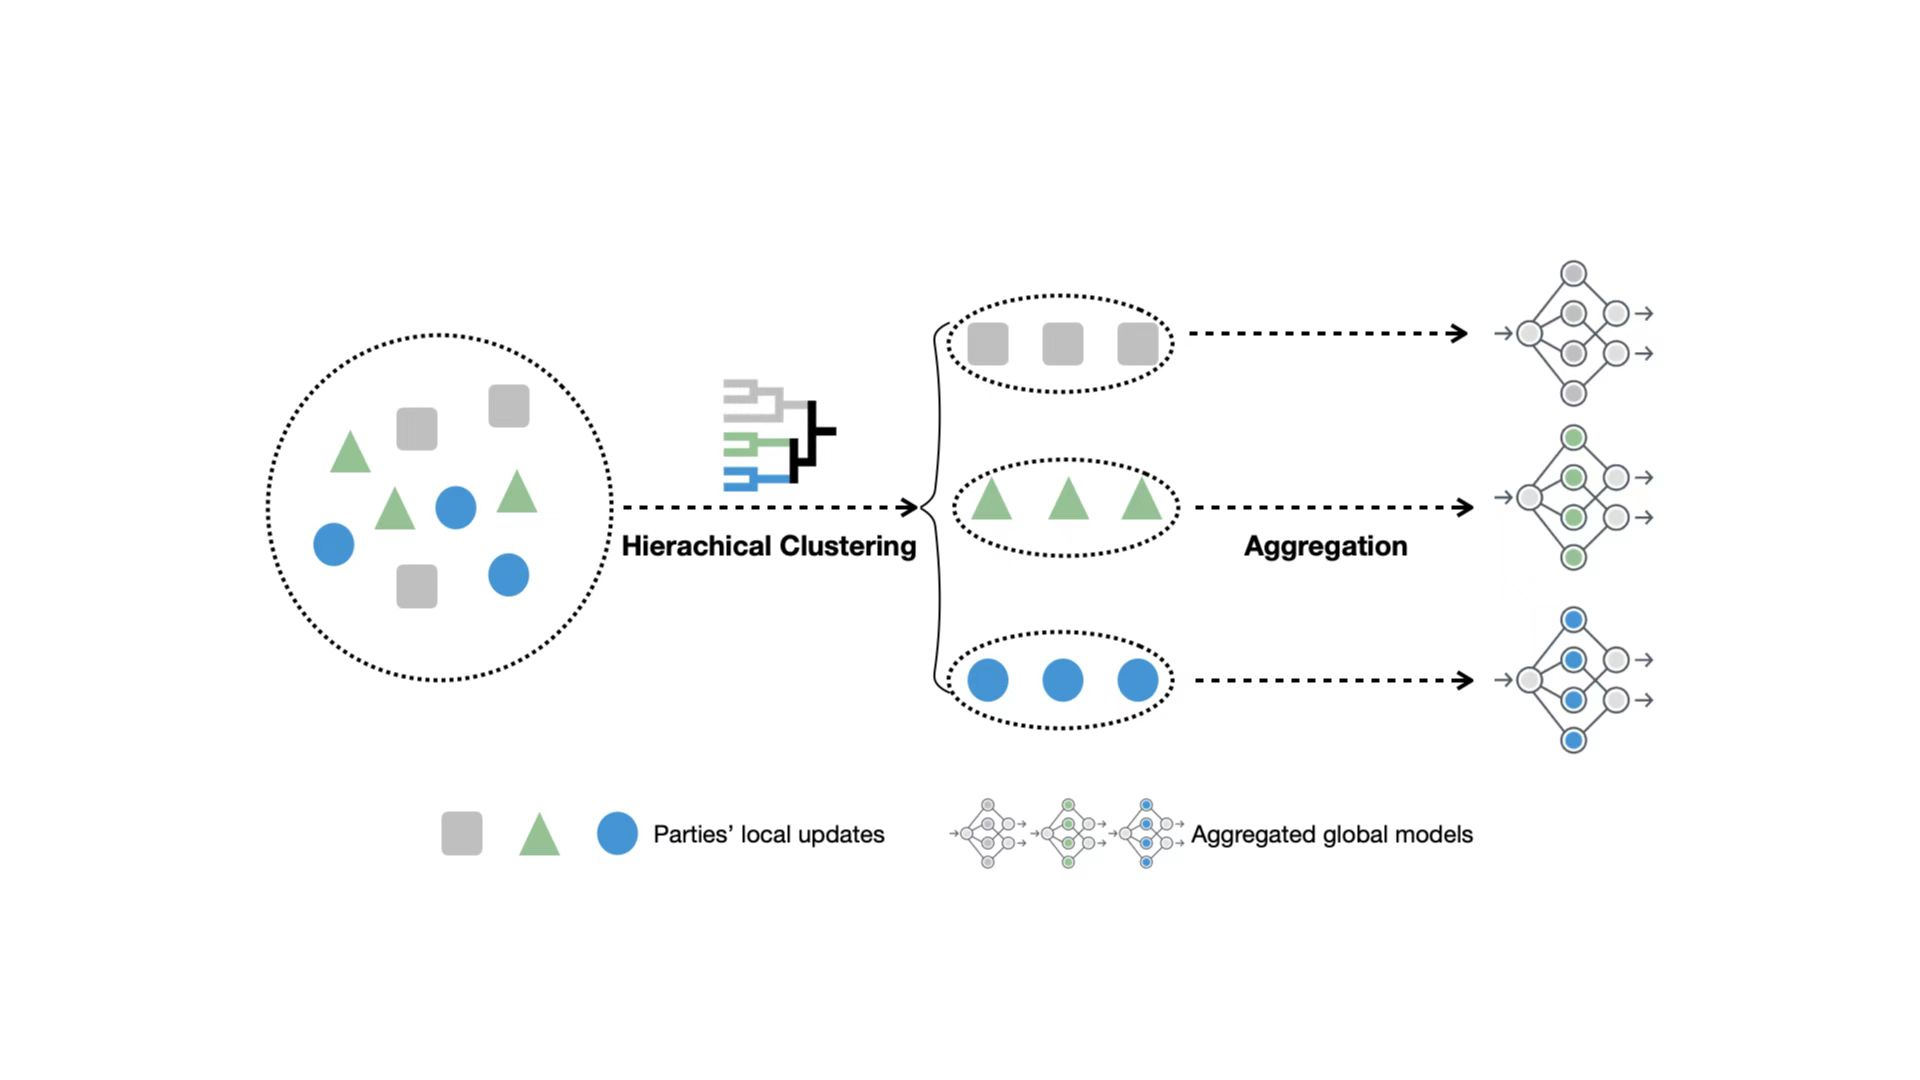
\includegraphics[scale=0.13]{figures/work2figs/hc.jpg}
        \caption{FL+HC简介}
        \label{hcjpg}
    \end{center}
\end{figure}

\subsection{密码技术介绍}

\subsubsection{加性秘密共享}
加性秘密共享是Shamir \cite{shamir1979share} 提出的一种安全多方计算技术。本章我们使用的是一种(2,2)的加性秘密共享方案,可用于安全两方计算(2PC)。这种方案可以在不同大小的环上做两方的安全计算,本章使用到的是两种特殊的环,环$\mathbb{Z}_2$和$\mathbb{p}, p=2^l$($l$一般为32)。当使用环$\mathbb{Z}_2$时,也被称为布尔秘密共享。
在布尔秘密共享方案中,布尔值$x \in \mathbb{Z}_2$可以被拆分为布尔共享份$\langle x\rangle_0^B$ 和 $\langle x\rangle_1^B$,其中三者满足$x = \langle x\rangle_0^B \oplus \langle x\rangle_0^B\;\text{mod}\;2$。
在使用环$x \in \mathbb{Z}_p$时,可以把环$\mathbb{Z}_p$上的元素$x$拆分为两个共享份$(\langle x\rangle_0, \langle x\rangle_1) = (r, x -r) \in \mathbb{Z}_p^2$, 其中$r$是在环$\mathbb{Z}_p$上随机采样得到的元素。通过执行安全的两方计算协议 \cite{rathee2020cryptflow2, rathee2021sirnn},在不重构出原始值的情况下,完成任意的算术运算。

\subsubsection{本章使用的安全两方计算(2PC)协议}
为了在共享份额上进行进行安全的计算,我们使用到了三种加性秘密共享上的基本运算 \cite{rathee2021sirnn},其基本信息的描述如下:
\begin{compactitem}
    \item \textbf{安全两方有符号数乘法}(Signed Value Multiplication,$\mathcal{F}_{\text{SMul}}$): 有符号数乘法 $(\mathcal{F}_{\text{SMul}})$ 以两方上的共享份额 $\langle x\rangle$ 以及 $\langle y\rangle$ 作为输入,然后输出 $\langle z\rangle$,其中三者满足:$z = x \times y$。
    \item \textbf{安全两方多路选择器}(Multiplexer,$\mathcal{F}_{\text{MUX}}$): 多路选择器 $(\mathcal{F}_{\text{MUX}})$ 以 $\langle x\rangle^B$ 和 $\langle y\rangle$ 作为输入,然后输出 $\langle z\rangle$,其中如果$x = 1$,则输出的$z$满足$z = y$,否则满足$z = 0$。 
    \item \textbf{安全两方DRelu} $(\mathcal{F}_{\text{DRelu}})$: DRelu 函数 $(\mathcal{F}_{\text{DRelu}})$ 以 $\langle x\rangle$ 作为输入,然后输出 $\langle z\rangle^B$,其中如果$x \geq 0$,则输出的$z$满足 $z = 1$,否则满足 $z = 0$。
\end{compactitem}

\subsubsection{伪随机生成技术}
伪随机生成技术(Pseudorandom Generator, PRG)\cite{yao1982theory} 可以根据一个均匀分布的随机数种子,生成一串很长的伪随机字符。只要这个随机数种子不被敌对方窃取,就能保证生成的这段随机字符,无法在多项式时间内与均匀分布采样出来的字符串做出区分。本章方案使用伪随机生成技术在参数上传和分发阶段保证参数隐私的同时,减少一半的通信开销(细节见\ref{4-framework})。

\section{问题描述}\label{4-problem}
本节我们主要对本章设计的的面向异质数据的隐私梯度聚合方案的系统模型、威胁模型以及设计目标,进行展开描述。

\subsection{系统模型}
本章设计的的面向异质数据的隐私保护梯度聚合方案系统模型如图\ref{sysjpg}所示。图中有$n$个参与方$P_1,P_2,...,P_n$和两个不共谋的服务器(FL服务提供商(SP)和计算服务器(CS)),这种实体分布在相似的研究\cite{liu2021privacy, dong2021flod, hao2021efficient}中非常常见。SP主导整个联合学习过程,而CS在必要的时机协助SP完成秘密共享份额上的安全两方计算(2PC),每个参与方$P$拥有用于联合训练的本地数据集$D$(用户间的数据分布时异质的),每个参与方的目标是联合与其有着同样学习目标的其他参与方(即数据分布一致),联合训练得到性能更好的全局模型。本章方案主要有以下三个步骤:
\begin{compactenum}
    \item SP将本轮全局模型广播给对应的用户。
    \item 每个参与方$P$将收到的全局模型应用到本地,然后利用本地数据$D$来更新模型参数,最后将更新梯度加密后发送给SP。
    \item 最后SP联合CS进行根据层次聚类结果,利用2PC协议进行安全的梯度聚合。
\end{compactenum}


\begin{figure}[htbp]
    \begin{center}
        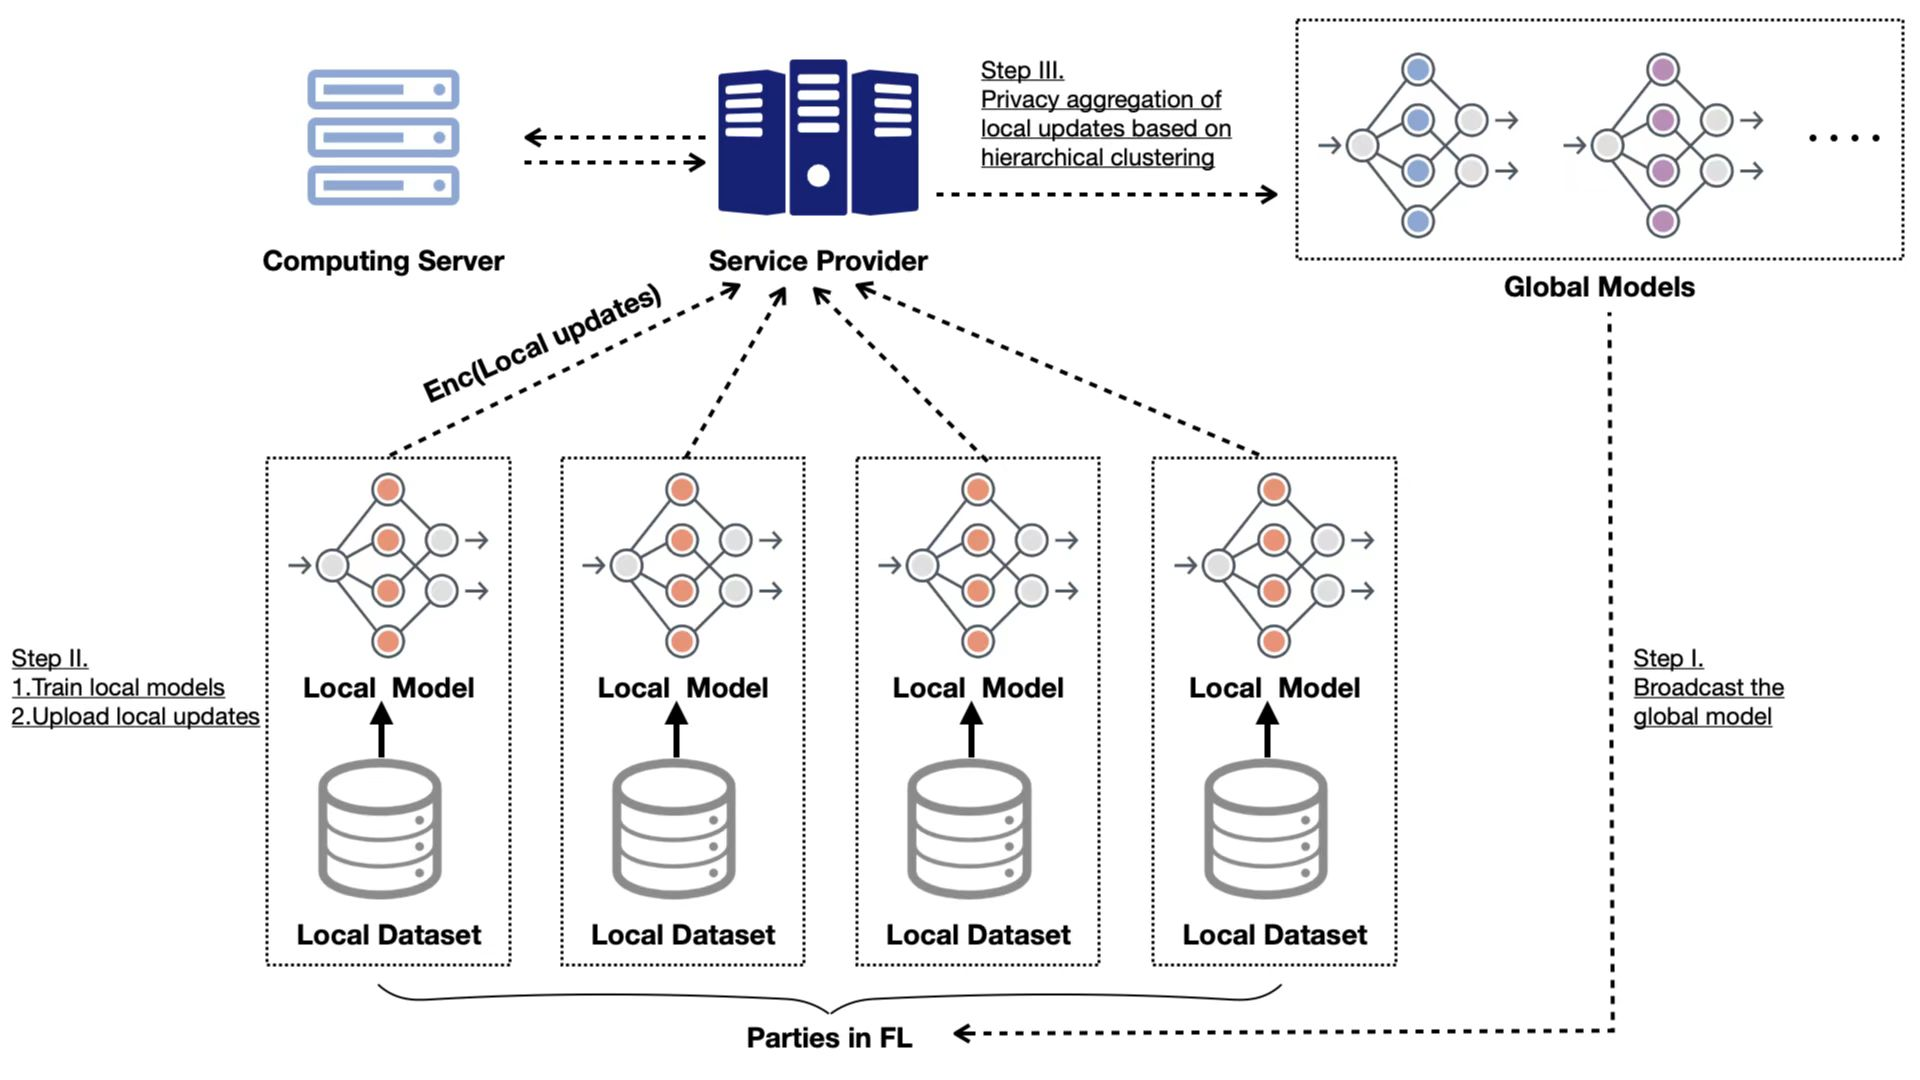
\includegraphics[scale=0.13]{figures/work2figs/system-model.jpg}
        \caption{方案系统模型图}
        \label{sysjpg}
    \end{center}
\end{figure}

\subsection{威胁模型}
在本章方案中,我们将服务器(SP和CS)视为诚实且好奇的,这意味着SP和CS将严格执行我们设计的安全协议,但是会主动的尝试推断用户的隐私信息。除此之外,我们还假设,SP和CS因为害怕公信力的丧失,不会发生共谋行为,这可以保证我们按照(2,2)加性秘密共享上传的用户梯度不会泄露给服务器。这个威胁模型是可以在真实世界满足的,并且在类似工作\cite{nguyen2022flame}中也用到了同样的威胁模型。比如说,Google和Amazon两种服务提供商,为了维护自己的信誉,都会选择正确执行我们设计的安全协议,而不是共谋获取用户的隐私信息。

\subsection{设计目标}
本章的目标是在保证用户梯度隐私的同时,提升FL在面对异质数据的联合训练性能。具体来说,我们的设计目标如下:
\begin{compactitem}
    \item \textbf{梯度隐私保护:}我们致力于实现对梯度的完全隐私保护,其中包括对用户上传的本地梯度的隐私保护,以及聚合之后的全局梯度的隐私保护。
    \item \textbf{异质数据准确率提升:}我们通过实现对梯度共享份上的安全层次聚类,来提升FL在面对异质数据的联合训练性能下降问题。
    \item \textbf{高效的安全计算协议:}我们精心设计了2PC协议,保证在聚类以及聚合结果正确性的同时,尽量减小计算和通信的复杂度。
\end{compactitem}

\section{基于秘密共享的隐私保护计算模块}\label{4-building}
%介绍为什么要设计这几个模块
为了对$n$个参与方的梯度向量的共享份$\{\boldsymbol{\langle g_1\rangle}, \boldsymbol{\langle g_2\rangle},...,\boldsymbol{\langle g_n\rangle} \}$进行安全的层次聚类操作,最首要的工作就是度量梯度向量之间的相似性,在层次聚类中,度量方式有欧式距离、曼哈顿距离以及余弦相似度,鉴于余弦相似度计算涉及到的开方和除法在共享份上的计算开销较大,本章仅考虑安全的欧式距离计算和安全的曼哈顿距离计算,最后提出了基于安全距离度量的安全层次聚类算法。

为了更好的理解我们提出的安全算法,本章使用到的符号对应的描述见表\ref{table-sym}。

\begin{table}
	\centering
	\caption{符号说明}
	\label{table-sym}
	\scalebox{0.95}{
		\renewcommand{\arraystretch}{1.2}
		\begin{tabular}{cl}
			\hline
			\hline
			\textbf{符号}               & \textbf{描述}                      \\
			\hline
			$\boldsymbol{g_i}$                          & 参与方 $P_i$ 的本地梯度向量      \\
			$\boldsymbol{G_x}$                          & 聚类结果中簇 $c_x$ 的全局梯度向量     \\
			$\boldsymbol{\langle g_i\rangle}$           & $\boldsymbol{g_i}$ 的共享份,其中 \\
			& SP 持有 $\boldsymbol{\langle g_i\rangle_0}$,CS 持有$\boldsymbol{\langle g_i\rangle_1}$ \\
			$\mathcal{D}_i$                & 参与方 $P_i$ 的本地数据集             \\
			$\textit{EDis}$                & 欧式距离(Euclidean distance)                        \\ 
			$\textit{MDis}$                & 曼哈顿距离(Manhattan distance)                        \\
			\hline
			\hline
		\end{tabular}
	}
\end{table}

\subsection{安全欧式距离计算}
为了安全的计算共享梯度向量$\boldsymbol{\langle g_i\rangle}$和$\boldsymbol{\langle g_j\rangle}$之间的欧式距离$\Vert \boldsymbol{g_i} - \boldsymbol{g_j} \Vert_2$,我们设计了安全的欧式距离(Secure Euclidean Distance, SED)计算算法。
首先SP和CS在本地计算$\boldsymbol{\langle z\rangle} = \boldsymbol{\langle g_i\rangle} - \boldsymbol{\langle g_j\rangle}$,然后SP和CS对于两个向量中的每一个元素协同调用$\mathcal{F}_{\text {SMul}}$,其中SP的输i入是$\boldsymbol{\langle z\rangle_0}[i]$,CS的输入是$\boldsymbol{\langle z\rangle_1}[i]$,然后SP和CS得到乘法的计算结果的共享份$\boldsymbol{\langle d\rangle}[i]$。
接下来SP和CS在本地计算向量$\boldsymbol{\langle d\rangle}$所有元素的内部和$\sum_{i=1}^{m} \boldsymbol{\langle d\rangle}[i]$,得到欧式距离平方的共享份$\langle \textit{EDis}^2\rangle$。
最后CS将共享份额$\langle \textit{EDis}^2\rangle_1$发送给SP,SP完成重构得到欧式距离明文$\textit{EDis}$(这个解密行为不会侵犯用户数据隐私,见第\ref{smd}节中的讨论)。
通过运行SED,SP和CS可以在不泄漏$\boldsymbol{g_i}$和$\boldsymbol{g_j}$每一个元素的情况下,得到梯度之间的欧式距离$\textit{EDis}$。SED算法的细节描述如算法\ref{alg1}所示。

\begin{algorithm}[htbp]
    \caption{安全欧式距离计算\\$\text{SED}(\boldsymbol{\langle g_i\rangle}, \boldsymbol{\langle g_j\rangle}) \xrightarrow{} \textit{EDis}$}
    \label{alg1}
    % \renewcommand{\algorithmicrequire}{\textbf{Input:}}
    % \renewcommand{\algorithmicensure}{\textbf{Output:}}
    \begin{algorithmic}[1]
    \REQUIRE SP拥有$\boldsymbol{\langle g_i\rangle_0}$和$\boldsymbol{\langle g_j\rangle_0}$, CS拥有$\boldsymbol{\langle g_i\rangle_1}$和$\boldsymbol{\langle g_j\rangle_1}$。 $\mathcal{F}_{\text {SMul}}$在文献\cite{rathee2021sirnn}中提出。
    \ENSURE $\boldsymbol{g_i}$和$\boldsymbol{g_j}$之间的欧式距离$\textit{EDis}$。
    % content
    \STATE SP本地计算$\boldsymbol{\langle z\rangle_0} = \boldsymbol{\langle g_i\rangle_0} - \boldsymbol{\langle g_j\rangle_0}$
    \STATE CS本地计算$\boldsymbol{\langle z\rangle_1} = \boldsymbol{\langle g_i\rangle_1} - \boldsymbol{\langle g_j\rangle_1}$
    % \STATE $\mathcal{F}_{\text {SMul }}(\langle z\rangle, \langle z\rangle)$
%    \FOR[$m$是$\boldsymbol{g_i}$的维度]{$i \in 1\:\textbf{to}\:m$} %\COMMENT{$m$ is the dimension of $\boldsymbol{g_i}$}
%        \STATE SP和CS调用函数$\mathcal{F}_{\text {SMul}}$, 其中SP的输入是$\boldsymbol{\langle z\rangle_0}[i]$,而CS的输入是 $\boldsymbol{\langle z\rangle_1}[i]$. 运算结束后SP和CS分别得到乘法结果的共享份$\boldsymbol{\langle d\rangle_0}[i]$ 和 $\boldsymbol{\langle d\rangle_1}[i]$。
%        % \STATE $(\lrangle EDis[i]\rangle,angle EDis[i]\rangle = \mathcal{F}_{\text {SMul }}(\langle z\rangle[i], \langle z\rangle[i])$
%    \ENDFOR
    \STATE SP和CS调用函数$\mathcal{F}_{\text {SMul}}$,其中两个乘数都是SP和CS持有的共享份$\boldsymbol{\langle z\rangle}$,计算得到乘法结果的共享份$\boldsymbol{\langle d\rangle}$ \COMMENT{对向量$\boldsymbol{\langle z\rangle}$中的元素逐个调用$\mathcal{F}_{\text {SMul}}$}
    \STATE SP本地计算$\langle \textit{EDis}^2\rangle_0 = \sum_{i=1}^{m} \boldsymbol{\langle d\rangle_0}[i]$
    \STATE CS本地计算$\langle \textit{EDis}^2\rangle_1 = \sum_{i=1}^{m} \boldsymbol{\langle d\rangle_1}[i]$
    \STATE CS发送$\langle \textit{EDis}^2\rangle_1$给SP, SP重构$\textit{EDis}^2 = \langle \textit{EDis}^2\rangle_0 + \langle \textit{EDis}^2\rangle_1$然后开方得到$\textit{EDis}$。
    \RETURN SP得到欧氏距离$\textit{EDis}$。
    \end{algorithmic}
\end{algorithm}

\subsection{安全曼哈顿距离计算}\label{smd}
为了安全的计算共享梯度向量$\boldsymbol{\langle g_i\rangle}$和$\boldsymbol{\langle g_j\rangle}$之间的曼哈顿距离$\norm{\boldsymbol{g_i} - \boldsymbol{g_j}}_1$,我们设计了安全的曼哈顿距离(Secure Manhattan Distance, SMD)计算算法。
首先SP和CS在本地计算$\boldsymbol{\langle z\rangle} = \boldsymbol{\langle g_i\rangle} - \boldsymbol{\langle g_j\rangle}$,然后SP联合CS以共享份$\boldsymbol{\langle z\rangle}$为输入,调用函数$\mathcal{F}_{\text {SMul}}$,计算得到DRelu值的布尔共享份$\boldsymbol{\langle y\rangle}^{B}$。
接着SP和CS分别计算$\boldsymbol{\langle \widetilde{y} \rangle_0}^{B} = \boldsymbol{\langle y\rangle_0}^{B}$和$\boldsymbol{\langle \widetilde{y} \rangle_1}^{B} = \boldsymbol{\langle y\rangle_1}^{B} \oplus 1$,得到DRelu结果对应的布尔取反结果$\boldsymbol{\langle \widetilde{y} \rangle}^{B}$。
紧接着SP和CS调用两次安全多路选择器,分别以$\{\boldsymbol{\langle z\rangle}, \boldsymbol{\langle y\rangle}^{B}\}$、$\{\boldsymbol{\langle z\rangle}, \boldsymbol{\langle \widetilde{y}\rangle}^{B}\}$为输入,获取$\boldsymbol{\langle z\rangle}$中的正数集合$\boldsymbol{
	\langle d_p\rangle}$以及负数集合$\boldsymbol{
	\langle d_n\rangle}$。
最后SP和CS在本地计算$\langle \textit{MDis}\rangle = \sum_{i=1}^{m}\boldsymbol{\langle d_p\rangle}[i] - \sum_{i=1}^{m}\boldsymbol{\langle d_n\rangle}[i]$,CS将结果共享份$\langle \textit{MDis}\rangle_1$发送给SP,SP完成重构得到曼哈顿距离$\textit{MDis}$。
SMD具体的算法细节描述如算法\ref{alg2}所示。

\textbf{讨论:}在我们的安全欧式距离以及安全的曼哈顿距离计算中,都将最后的结果($\langle \textit{EDis}\rangle$和$\langle \textit{MDis}\rangle$)从共享份重构为明文($\textit{EDis}$和$\textit{MDis}$),我们认为这个距离信息的重构不会侵犯用户的数据隐私。
很明显即使SP能够得到任意两个梯度之间的距离信息,也无法推断出任何一个梯度的具体信息,包括梯度的大小、方向以及单个元素的正负。文献\cite{geiping2020inverting}提出的针对梯度的数据重构方案,可以根据梯度之间的余弦相似度,重构用户的训练样本,但是这个方案需要知道梯度的正负,而在我们的方案中,SP是无法获取这个信息的,所以是无法泄露用户的数据隐私的。

\begin{algorithm}[htbp]
    \caption{安全曼哈顿距离计算\\$\text{SMD}(\boldsymbol{\langle g_i\rangle}, \boldsymbol{\langle g_j\rangle}) \xrightarrow{} \textit{MDis}$}
    \label{alg2}
    \begin{algorithmic}[1]
    % \renewcommand{\algorithmicrequire}{\textbf{Input:}}
    % \renewcommand{\algorithmicensure}{\textbf{Output:}}
    \REQUIRE SP 拥有 $\boldsymbol{\langle g_i\rangle_0}$ 和 $\boldsymbol{\langle g_j\rangle_0}$, CS 拥有 $\boldsymbol{\langle g_i\rangle_1}$ 和 $\boldsymbol{\langle g_j\rangle_1}$. $\mathcal{F}_{\text {DRelu}}$ 和 $\mathcal{F}_{\text {MUX}}$ 在文献\cite{rathee2021sirnn}中提出。
    \ENSURE $\boldsymbol{g_i}$ 与 $\boldsymbol{g_j}$之间的曼哈顿距离$\textit{MDis}$。
    % content
    \STATE SP 本地计算 $\boldsymbol{\langle z\rangle_0} = \boldsymbol{\langle g_i\rangle_0} - \boldsymbol{\langle g_j\rangle_0}$
    \STATE CS 本地计算 $\boldsymbol{\langle z\rangle_1} = \boldsymbol{\langle g_i\rangle_1} - \boldsymbol{\langle g_j\rangle_1}$
    \STATE SP 和 CS 调用 $\mathcal{F}_{\text{DRelu}}$,其中输入为SP和CS持有的共享份$\boldsymbol{\langle z\rangle}$,计算得到DRelu值的布尔共享份$\boldsymbol{\langle y\rangle}^{B}$。
    \STATE SP 和 CS 分别调用 $\boldsymbol{\langle \widetilde{y} \rangle_0}^{B} = \boldsymbol{\langle y\rangle_0}^{B}$ 和 $\boldsymbol{\langle \widetilde{y} \rangle_1}^{B} = \boldsymbol{\langle y\rangle_1}^{B} \oplus 1$。\COMMENT{安全的获得布尔共享份$\boldsymbol{\langle y\rangle}^{B}$的取反结果$\boldsymbol{\langle \widetilde{y} \rangle}^{B}$。}
    % \State SP sets $\boldsymbol{\langle \widetilde{g_i}\rangle_0}$ = - $\boldsymbol{\langle g_i\rangle_0}$ and $\boldsymbol{\langle \widetilde{g_j}\rangle_0}$ = - $\boldsymbol{\langle g_j\rangle_0}$
    % \State CS sets $\boldsymbol{\langle \widetilde{g_i}\rangle_1}$ = - $\boldsymbol{\langle g_i\rangle_1}$ and $\boldsymbol{\langle \widetilde{g_j}\rangle_1}$ = - $\boldsymbol{\langle g_j\rangle_1}$
    % \For{$i \in [1...m]$} \Comment{$m$ is the dimension of $\boldsymbol{g_i}$}
        \STATE SP 和 CS 调用 $\mathcal{F}_{\text{MUX}}$,其中输入为SP和CS持有的共享份$\boldsymbol{\langle z\rangle}$ 和 $\boldsymbol{\langle y\rangle}^{B}$,计算得到$\boldsymbol{\langle z\rangle}$中的正数集合$\boldsymbol{
        \langle d_p\rangle}$。
        \STATE SP 和 CS 调用 $\mathcal{F}_{\text{MUX}}$,其中输入为SP和CS持有的共享份 $\boldsymbol{\langle z\rangle}$ 和 $\boldsymbol{\langle \widetilde{y}\rangle}^{B}$,计算得到$\boldsymbol{\langle z\rangle}$中的负数集合$\boldsymbol{
        \langle d_n\rangle}$
    % \EndFor
    \STATE SP 本地计算 $\langle \textit{MDis}\rangle_0 = \sum_{i=1}^{m}\boldsymbol{\langle d_p\rangle_0}[i] - \sum_{i=1}^{m}\boldsymbol{\langle d_n\rangle_0}[i]$ \COMMENT{$m$ 是 $\boldsymbol{g_i}$的维度}
    \STATE CS 本地计算 $\langle \textit{MDis}\rangle_1 = \sum_{i=1}^{m}\boldsymbol{\langle d_p\rangle_1}[i] - \sum_{i=1}^{m}\boldsymbol{\langle d_n\rangle_1}[i]$
    \STATE CS 发送 $\langle \textit{MDis}\rangle_1$ 给 SP,然后SP 重构出 $\textit{MDis} = \langle \textit{MDis}\rangle_0 + \langle \textit{MDis}\rangle_1$。
    \RETURN SP得到曼哈顿距离$\textit{MDis}$。
    \end{algorithmic}
\end{algorithm}

\subsection{安全的梯度层次聚类}
%写随机梯度裁剪
为了完成对共享份梯度集合$\{\boldsymbol{\langle g_1\rangle}, \boldsymbol{\langle g_2\rangle},...,\boldsymbol{\langle g_n\rangle} \}$的安全层次聚类,我们将整个聚类过程划分为三个阶段:
\begin{compactenum}
	\item \textbf{梯度的随机降维:}考虑到神经网络梯度的维度较高,而对梯度的层次聚类不使用全部维度也能保证较高的准确性(实验验证参考\ref{4-exp}),我们对梯度进行了随机降维操作,随机抽取一部分元素,对所有的梯度向量 $\{\boldsymbol{\langle g_1\rangle}, \boldsymbol{\langle g_2\rangle},...,\boldsymbol{\langle g_n\rangle} \}$ 抽取相同下标的一部分元素,得到降维后的梯度向量 $\{\dot{\boldsymbol{\langle g_1\rangle}}, \dot{\boldsymbol{\langle g_2\rangle}},...,\dot{\boldsymbol{\langle g_n\rangle}} \}$。
	\item \textbf{梯度间距离矩阵计算:}这一阶段完成每个共享梯度向量$\dot{\svec{g_i}}$,与其它$n-1$个梯度的距离计算,得到一个距离矩阵$\{\textit{Dis}_{11}, \textit{Dis}_{12},...,\textit{Dis}_{nn}\}$,其中距离的计算过程以梯度共享份为输入,调用上述SED或SMD安全距离计算算法,在保证梯度隐私的前提下,得到明文的距离矩阵。
	\item \textbf{基于距离矩阵的聚类过程:}在得到预先计算好的距离矩阵之后,再搭配其它层次聚类参数,比如不同的簇间距离计算方式($avg, min\; or\; max$)以及距离阈值,完成对梯度的自底向上的层次聚类。
\end{compactenum}
具体的层次聚类算法细节如算法\ref{alg3}所示。

\begin{algorithm}[htbp]
	\caption{安全的梯度层次聚类算法 \\ $\text{SHC}(\{\boldsymbol{\langle g_1\rangle}, \boldsymbol{\langle g_2\rangle},...,\boldsymbol{\langle g_n\rangle} \}) \rightarrow \{c_1,c_2,...,c_l \}$}
	\label{alg3}
	\begin{algorithmic}[1]
		\REQUIRE SP 和 CS 拥有$\{\boldsymbol{\langle g_1\rangle}, \boldsymbol{\langle g_2\rangle},...,\boldsymbol{\langle g_n\rangle} \}$。 \COMMENT{$n$ 表示参与方数量}
		\ENSURE $l$ 个簇 $\{c_1,c_2,...,c_l \}$。
		% content
		\STATE SP 和 CS 对梯度共享份 $\{\boldsymbol{\langle g_1\rangle}, \boldsymbol{\langle g_2\rangle},...,\boldsymbol{\langle g_n\rangle} \}$ 进行随机降维得到:\\ $\{\dot{\boldsymbol{\langle g_1\rangle}}, \dot{\boldsymbol{\langle g_2\rangle}},...,\dot{\boldsymbol{\langle g_n\rangle}} \}$
		\FOR{$i \gets 1\:\textbf{to}\:n$}
		\FOR{$j \gets 1\:\textbf{to}\:n$}
			\STATE SP 和 CS 调用$\textit{Dis}_{ij} \xleftarrow{}\text{SMD}(\dot{\boldsymbol{\langle g_i\rangle}}, \dot{\boldsymbol{\langle g_j\rangle}})$ (或者 $\text{SED}\dot{\boldsymbol{\langle g_i\rangle}}, \dot{\boldsymbol{\langle g_j\rangle}})$), 然后SP获得距离值$\textit{Dis}_{ij}$。
		\ENDFOR
		\ENDFOR
		\STATE $\{c_1,c_2,...,c_l \} \xleftarrow{} \textsc{Clustering}(\textit{Dis}_{11},...,\textit{Dis}_{nn})$ \COMMENT{基于预计算距离矩阵的层次聚类}
		\RETURN SP和CS获得层次聚类结果 $\{c_1,c_2,...,c_l \}$。
	\end{algorithmic}
\end{algorithm}


\section{面向异质数据的隐私保护梯度聚合方案}\label{4-framework}
基于\ref{4-building}节设计的相关安全计算模块,本节介绍我们设计的面向异质数据的隐私保护梯度聚合方案,在FL+HC\cite{briggs2020federated}的基础上,赋予了完全的梯度隐私保护能力。
本节首先介绍对方案的概述,然后具体阐述方案的四个阶段:初始化阶段、本地梯度的生成和编码阶段、梯度的安全聚和阶段以及梯度的安全分发阶段。在整个方案中,用户上传的梯度信息以及聚合生成的全局梯度,都不会被SP以及CS窃取,实现了对梯度的完全隐私保护。

\subsection{方案概述}
参与方$P_i$在本地生成梯度之后,利用文献\cite{hao2021efficient}的方法,我们只用向SP上传一份梯度$\svec{g_i}$,另一份梯度由$P_i$和CS利用相同的随机数种子(在初始化阶段协商),借助伪随机算法PRG生成,以此减少一半的通信开销。
在梯度的聚合阶段,SP和CS在聚类轮次执行一次安全的梯度层次聚类,然后根据聚类结果来聚合梯度,对于聚类轮次之前的轮次,所有的参与方被视为一个簇。
最后SP和CS完成对聚合梯度的安全分发,保证全局梯度的隐私。

\subsection{具体方案}
本节具体介绍方案涉及到的四个阶段。%TODO add frame flow.

\subsubsection{初始化阶段}
本阶段在整个方案中只会被执行一次。利用文献\cite{diffie2022new}提出的Diffie-Hellman密钥协商协议,每个参与方$P_i$与CS协商一个私有的种子密钥$k_i^{seed}$。这个密钥在本地梯度的上传以及全局梯度的分发过程中,保证参与方$P_i$与CS能够非交互的生成同样的随机向量,具体细节见阶段\ref{local}和阶段\ref{distribution}。

\subsubsection{本地梯度的生成和编码阶段}\label{local}
本阶段描述参与方$P_i$如何生成本地梯度的共享份$\svec{g_i}$,包括上传给SP的共享份$\svec[0]{g_i}$,以及与CS协同生成的共享份$\svec[1]{g_i}$。

首先,参与方$P_i$利用收到的全局梯度更新本地模型,再使用本地数据$\mathcal{D}_i$训练模型得到本地的原始更新,是一个浮点数梯度向量$\overline{\bs{g_i}}$。
为了将浮点梯度$\overline{\bs{g_i}}$表示为环 $\mathbb{Z}_p$($p=2^l$,$l$表示比特长度)上的共享份,我们首先要对这个向量进行定点数编码。
对于浮点数 $v$ 来说,我们使用的定点编码操作如下:
\begin{equation}
	Encode(v) = \lfloor 2^s \times v\rfloor \;\text{mod}\;p
\end{equation}
其中 $\lfloor v\rfloor$表示小于等于浮点数 $v$ 的最大整数值,而 $s$ 表示定点数的精度。
对浮点向量 $\overline{\bs{g_i}}$ 中的每个元素都进行定点编码,于是就得到了本地梯度的定点表示:
\begin{equation}
	\boldsymbol{g_i} = Encode(\overline{\boldsymbol{g_i}})
\end{equation}
然后参与方$P_i$使用PRG技术,利用随机数种子 $k_i^{seed}$生成随机向量 $\bs{r_i}$,然后将属于SP的梯度共享份 $\svec[0]{g_i} = \bs{g_i} - \bs{r_i}$ 发送给SP。为了提升通信效率,我们让CS在本地使用同样的随机数种子 $k_i^{seed}$ 生成相同的随机变量 $\bs{r_i}$,所以属于CS的梯度共享份为 $\svec[1]{g_i} = \bs{r_i}$,这种方式减少了本方案在梯度上传过程中一半的通信开销。

\subsubsection{梯度的安全聚合阶段}
在FL+HC \cite{briggs2020federated}中,会在特定的轮次 $t$ 进行梯度的层次聚类操作,在轮次 $t$ 之前,所有的参与方被视为一个簇,联合生成一个全局梯度(与FedAvg \cite{mcmahan2017communication} 一致)。当进行到第$t$轮时,我们对所有的梯度执行安全的层次聚类操作:
\begin{equation}
	\{c_1,c_2,...,c_l \} \leftarrow \text{SHC}(\{\boldsymbol{\langle g_1\rangle}, \boldsymbol{\langle g_2\rangle},...,\boldsymbol{\langle g_n\rangle} \})
\end{equation}
得到聚类结果$\{c_1,c_2,...,c_l \}$后,对用一个簇中的所有参与方,进行线性聚合操作:
\begin{equation}
	\boldsymbol{\langle G_x\rangle} = \frac{\sum_{j \in c_x}\boldsymbol{\langle g_j\rangle}}{n_x}
\end{equation}
其中$j$ 表示簇 $c_x$ 中的参与方,$n_x$ 表示簇 $c_x$ 中参与方的数量,$\svec{G_x}$ 表示聚合之后的全局梯度,以此我们就得到了所有的全局聚合梯度的共享份 $\{\svec{G_1},\svec{G_2},...,\svec{G_l}\}$。


\subsubsection{梯度的安全广播阶段}\label{distribution} 
为了保证全局梯度 $\svec{G_x}$ 的隐私,我们没有选择让SP和CS重构出$\bs{G_x}$再广播给用户。而是设计了安全的参数分发算法,在不提升通信开销的同时,保证了全局梯度的隐私,算法细节描述如算法\ref{alg4}所示。首先参与方$P_i$ 和 CS利用$k_i^{seed}$协同相同的随机变量$\bs{r_i^{\prime}}$,然后CS使用该随机变量对梯度共享份进行扰动得到 $\svec[0]{\widehat{G_x}} = \svec[0]{G_x} + \bs{r_i^{\prime}}$,紧接着CS将 $\svec[0]{\widehat{G_x}}$ 发送给SP,SP重构扰动之后的全局梯度 $\boldsymbol{\widehat{G_x}} = \boldsymbol{\langle G_x\rangle_0} + \boldsymbol{\langle \widehat{G_x}\rangle_1}$,最后将 $\boldsymbol{\widehat{G_x}}$ 发送给 参与方$P_i$,$P_i$利用$r_i^{\prime}$消除扰动得到$\boldsymbol{G_x}$。

参与方$P_i$拿到全局梯度$\bs{G_x}$后,对梯度进行定点数解码操作:
\begin{equation}
	\bs{\overline{G_x}} = Decode(\bs{G_x})
\end{equation}
其中解码操作首先将元素$v$视为浮点数,然后除以$2^s$,得到对应的梯度浮点数。

\begin{algorithm}[htbp]
	\caption{安全的全局梯度广播 \\$\text{SGB}(\boldsymbol{\langle G_x\rangle}) \rightarrow \boldsymbol{G_x}$}
	\label{alg4}
	\begin{algorithmic}[1]
		\REQUIRE SP 和 CS 拥有参与方 $P_i$的全局梯度$\boldsymbol{\langle G_x\rangle}$.
		% clustering results $\{c_1,c_2,...,c_l\}$ and global gradients $\{\boldsymbol{\langle G_1\rangle,...,\langle G_l\rangle\}}$ \Comment{$l$ is the number of clusters}
		\ENSURE 参与方$P_i$ 获得相应的全局梯度$\boldsymbol{G_x}$
		% \Comment{$x$ indicates the cluster to which $P_i$ belongs}
		% content
		\STATE $P_i$ 与 CS 利用相同的随机数种子生成 $\boldsymbol{r_i}$ = PRG($k_i^{seed}$) \COMMENT{相同的$k_i^{seed}$ 保证了$\boldsymbol{r_i}$ 在 $P_i$ 和 CS之间的一致性}
		\STATE CS 扰动$\boldsymbol{\langle G_x\rangle_1}$:\\ $\boldsymbol{\langle \widehat{G_x}\rangle_1} = \boldsymbol{\langle G_x\rangle_1} + \boldsymbol{r_i}$
		\STATE CS 发送$\boldsymbol{\langle \widehat{G_x}\rangle_1}$ 给 SP, 然后 SP 重构扰动后的全局梯度 $\boldsymbol{\widehat{G_x}}$:\\ $\boldsymbol{\widehat{G_x}} = \boldsymbol{\langle G_x\rangle_0} + \boldsymbol{\langle \widehat{G_x}\rangle_1}$
		\STATE SP 发送 $\boldsymbol{\widehat{G_x}}$ 到 $P_i$, 然后 $P_i$ 消除全局梯度的扰动:\\$\boldsymbol{G_x} = \boldsymbol{\widehat{G_x}} - \boldsymbol{r_i}$
	\end{algorithmic}
\end{algorithm}

%option
\section{安全性分析}\label{4-analysis}
本方案的目标是保护参与方本地数据的隐私,以及聚合之后的全局梯度的隐私,本节对安全计算模块SED、SMD、SHC以及安全的全局梯度广播协议进行安全性分析,其中敌对方为半诚实的服务器SP和CS。

为了证明本方案的正确性,本节首先给出半诚实模型下的安全性定义,如定义\ref{sec-def}所示。

\begin{definition}[半诚实模型的安全性 \cite{bogdanov2008sharemind}]\label{sec-def}	
	对于安全计算协议 $\mathcal{F}$,我们将执行协议生成的输出称为真实视图。
	假设存在一个多项式概率模拟器 $\mathcal{S}$,可以生成均匀分布的随机数,我们称这个输出为模拟视图。如果真实世界中的敌对方 $\mathcal{A}$ 获取到了一份输出,在多项式时间内无法区分输出是由执行协议$\mathcal{F}$产生的真实视图,还是由模拟器 $\mathcal{S}$ 产生的模拟视图,则认为协议 $\mathcal{F}$ 是安全的。
\end{definition}

为了更好的证明协议的安全性,再引入如下引理:
\begin{lemma}\label{l1}
	如果构成协议的所有子协议在半诚实模型下都是安全的,则认为该协议在半诚实模型下是安全的\cite{bi2020design}。
\end{lemma}

\begin{lemma}\label{l2}
	如果$ a, b \in \mathbb{Z}_p$ 是随机均匀分布的,且 $a$ 与 $b$ 是相互独立的,那么 $a \pm b$ 的结果也是随机均匀分布的,并且与$a,b$相互独立\cite{bogdanov2008sharemind}。
\end{lemma}

\begin{theorem}
	本章提出的安全欧式距离计算协议\ref{alg1}(SED)在半诚实模型下是安全的。
\end{theorem}

\begin{proof}\label{p1}
	在SED协议中,SP获取到的真实视图为 $\{\svec[0]{z}, \svec[0]{d}, \langle \textit{EDis}^2\rangle_0\}$,其中 $\svec[0]{z}$ 是由独立的共享份相减得到,由引理\ref{l2}可知,$\svec[0]{z}$ 是随机均匀分布的。$\svec[0]{d}$ 是由SP和CS对$\svec{z}$协同调用$\mathcal{F}_{\text {SMul}}$得到,而 $\mathcal{F}_{\text {SMul}}$ 的安全性在文献 \cite{rathee2021sirnn} 中得到了证明。$\langle \textit{EDis}^2\rangle_0$ 是由随机均匀分布的向量 $\svec[0]{d}$ 对内部元素求和得到,由引理\ref{l2}可知$\langle \textit{EDis}^2\rangle_0$也是随机均匀分布的,因此结合引理\ref{l1},对于SP来说,无法在多项式时间内区分真实视图和由模拟器$\mathcal{S}$生成的模拟视图。同理,对于CS持有的真实视图 $\{\svec[1]{z}, \svec[1]{d}, \langle \textit{EDis}^2\rangle_1\}$,也无法区分于随机生成的模拟视图,所以SED协议在半诚实模型下是安全的。
\end{proof}

\begin{theorem}
	本章提出的安全曼哈顿距离计算协议\ref{alg2}(SMD)在半诚实模型下是安全的。
\end{theorem}

\begin{proof}\label{p2}
	在SMD协议中,SP得到的真实视图为 $\{\svec[0]{z}, \svec[0]{y}^B, \svec[0]{\widetilde{y}}^B, \svec[0]{d_p}, \svec[0]{d_n}\}$,其中$\svec[0]{z}$已由证明\ref{p1}证明是随机均匀分布的,而$\svec[0]{y}^B$是SP和CS协同调用函数 $\mathcal{F}_{\text {MUX}}$得到,$\mathcal{F}_{\text {MUX}}$的安全性已由文献\cite{rathee2021sirnn}证明。$\svec[0]{\widetilde{y}}^B$ 是 $\svec[0]{y}^B$ 的相反数,因为 $\svec[0]{y}^B$ 是随机均匀分布的,所以 $\svec[0]{\widetilde{y}}^B$ 也是随机均匀分布的。$\svec[0]{d_p}$ 与 $\svec[0]{d_n}$都是SP和CS运行协议$\mathcal{F}_{\text {MUX}}$的结果,其安全性已在文献\cite{rathee2021sirnn}中证明,综上结合引理\ref{l1},SP在多项式时间内无法区分真实视图和由模拟器$\mathcal{S}$生成的模拟视图。同理,对于CS收到的真实视图 $\{\svec[1]{z}, \svec[1]{y}^B, \svec[1]{\widetilde{y}}^B, \svec[1]{d_p}, \svec[1]{d_n}\}$,也无法区分于随机生成的模拟视图,所以SMD协议在半诚实模型下是安全的。
\end{proof}

\begin{theorem}
	本章提出的安全梯度层次聚类协议\ref{alg3}(SHC)在半诚实模型下是安全的。
\end{theorem}

\begin{proof}
	本章提出的SHC协议构建于SED和SMD协议之上,由于SED和SMD协议在半诚实模型下的安全性已经得到了证明(见证明\ref{p1}和证明\ref{p2}),所以结合引理\ref{l1},SHC协议在半诚实模型下也是安全的。
\end{proof}

\begin{theorem}
	本章提出的安全全局梯度广播协议\ref{alg4}(SGB)在半诚实模型下是安全的。
\end{theorem}

\begin{proof}
	在SGB协议中,SP收到的真实视图是$\{\boldsymbol{\langle \widehat{G_x}\rangle_1}, \boldsymbol{\widehat{G_x}}\}$,其中$\boldsymbol{\langle \widehat{G_x}\rangle_1}$是由共享份和随机向量相加得到,$\boldsymbol{\widehat{G_x}}$ 是由共享份和扰动过后的共享份相加得到,由引理\ref{l2}可知其都是随机均匀分布的,因此SP收到的真实视图与模拟器$\mathcal{S}$随机生成的模拟视图,是计算不可区分的。CS获得的真实视图是 $\{\boldsymbol{\langle G_x\rangle_1}, \bs{r_i}, \boldsymbol{\langle \widehat{G_x}\rangle_1}\}$,其中$\boldsymbol{\langle G_x\rangle_1}$是共享份,$\bs{r_i}$ 是生成的随机向量,都是随机且均匀分布的,而 $\boldsymbol{\langle \widehat{G_x}\rangle_1} = \boldsymbol{\langle G_x\rangle_1} + \bs{r_i}$ 由引理\ref{l2} 可知,其也是随机均匀分布的,所以SP和CS都无法区分真实视图与模拟器$\mathcal{S}$生成的模拟视图,因此安全的梯度广播协议在半诚实模型下是安全的。
\end{proof}

\section{实验评估}\label{4-exp}
本节我们通过在真实数据集上开展一系列实验,证明了本方案对异质数据联合训练带来的性能提升,同时也对本方案设计的2PC安全计算协议进行了性能评估。我们所有的实验都是在一台配置有Ubuntu 20.04, Intel(R) Core(TM) i9-10980XE CPU @ 3.00GHz CPU 和 64GB RAM 的主机上进行,其中参与方和服务器分别用不同的进程来模拟。

\subsection{实验配置}

\subsubsection{数据集和模型架构}
为了测试本方案在训练准确率上的表现,我们选择了两个经典的图像分类任务数据集:
\begin{compactitem}
	\item \textbf{MNIST数据集:}其训练集中包含 $60,000$ 张手写数字图片,图片内容是0-9的手写数字(共十类),每张图片有 $28 \times28$ 个像素,测试集中含有 $10,000$ 张格式相同的图片。
	\item \textbf{CIFAR-10数据集:}其训练集包含 $60,000$ 张彩色图片,每张图片大小为 $32 \times 32$ 个像素,其中 $50,000$ 张图片用于训练,$10,000$张图片用于测试,一共有十类图片,每类图片 $6000$ 张。
\end{compactitem}
对于MNIST数据集分类任务的训练模型网络,我们选择了最简单的两层全连接网络,其中第一层的参数规模为 $724 \times 100$,第二层的参数规模为 $100 \times 10$,一共大概 $80k$ 个参数。对于CIFAR-10数据集分类任务,我们使用了一个简单的卷积神经网络,来自于TensorFlow的官网教程 \footnote{web URL: https://www.tensorflow.org/tutorials/images/cnn?hl=en},其中包含三层卷积网络层和两层全连接层,一共有大约 $123k$ 个参数。

\subsubsection{异质数据(Non-IID)配置}
%TODO 描述一下和前面三种分类的对应关系
我们使用的Non-IID配置与FL+HC \cite{briggs2020federated} 一致,选用了两种较为极端的异质数据配置,具体配置信息如下:
\begin{compactenum}
	\item \textbf{分布偏差的异质数据:}这种异质数据分布首先由文献 \cite{mcmahan2017communication} 提出,用于模拟数据特征和数据标签极致偏移的情况,每个参与方仅仅持有两个标签的数据,如果参与方有$600$ 个样本,其中有 $300$ 个样本的标签为 $1$, 其余 $300$ 个样本的标签为 $2$,其它的参与方也仅持有两个标签的数据,且参与方之间的标签分布不一致。这种数据分布方式可以模拟数据特征分布偏差($\mathcal{P}_i(x) \neq \mathcal{P}_j(x)$)和数据标签分布偏差($\mathcal{P}_i(y) \neq \mathcal{P}_j(y)$)的情况。
	\item \textbf{标签交换的异质数据:}这种异质数据分布在文献 \cite{sattler2020clustered} 中提出,其将数据划分为四个组,对每个组随机挑选两个不同的标签交换。比如将$60,000$个样本划分给$100$个参与方,首先将 $60,000$个样本划分为四个组,每组 $15,000$个样本,对于这这些样本挑选两个标签比如3和9交换,即将所有标签为3的数据标签改为9,反之依然,然后再将这些样本均匀划分到 $25$ 个参与方。这种划分方式用于模拟数据标注概念偏差的情况,即 $\mathcal{P}(y \mid x)$ 在参与方中不同的情况。
\end{compactenum}

\subsubsection{超参数}
%TODO 2PC实验超参数搞一搞
对于每个本地训练任务,我们把批大小($batch\;size$)设置为 $2^7$,随机梯度下降算法(SGD)的动量(momentum)设置为 $0.9$,初始化学习率设为 $0.1$。
对于2PC计算协议中的超参数,我们将环$\mathbb{Z}_p$ 的初始化大小 $p$ 设置为 $2^{32}$,定点数编码的缩放量设置为 $2^6$。

\subsection{实验结果}
\begin{figure}[htb]
	\centering
	\subfloat[MNIST数据集在分布偏差的异质数据下,随训练轮次以及聚类轮次变化的的测试准确率]{
		\begin{minipage}[b]{0.27\textwidth}
			\centering
			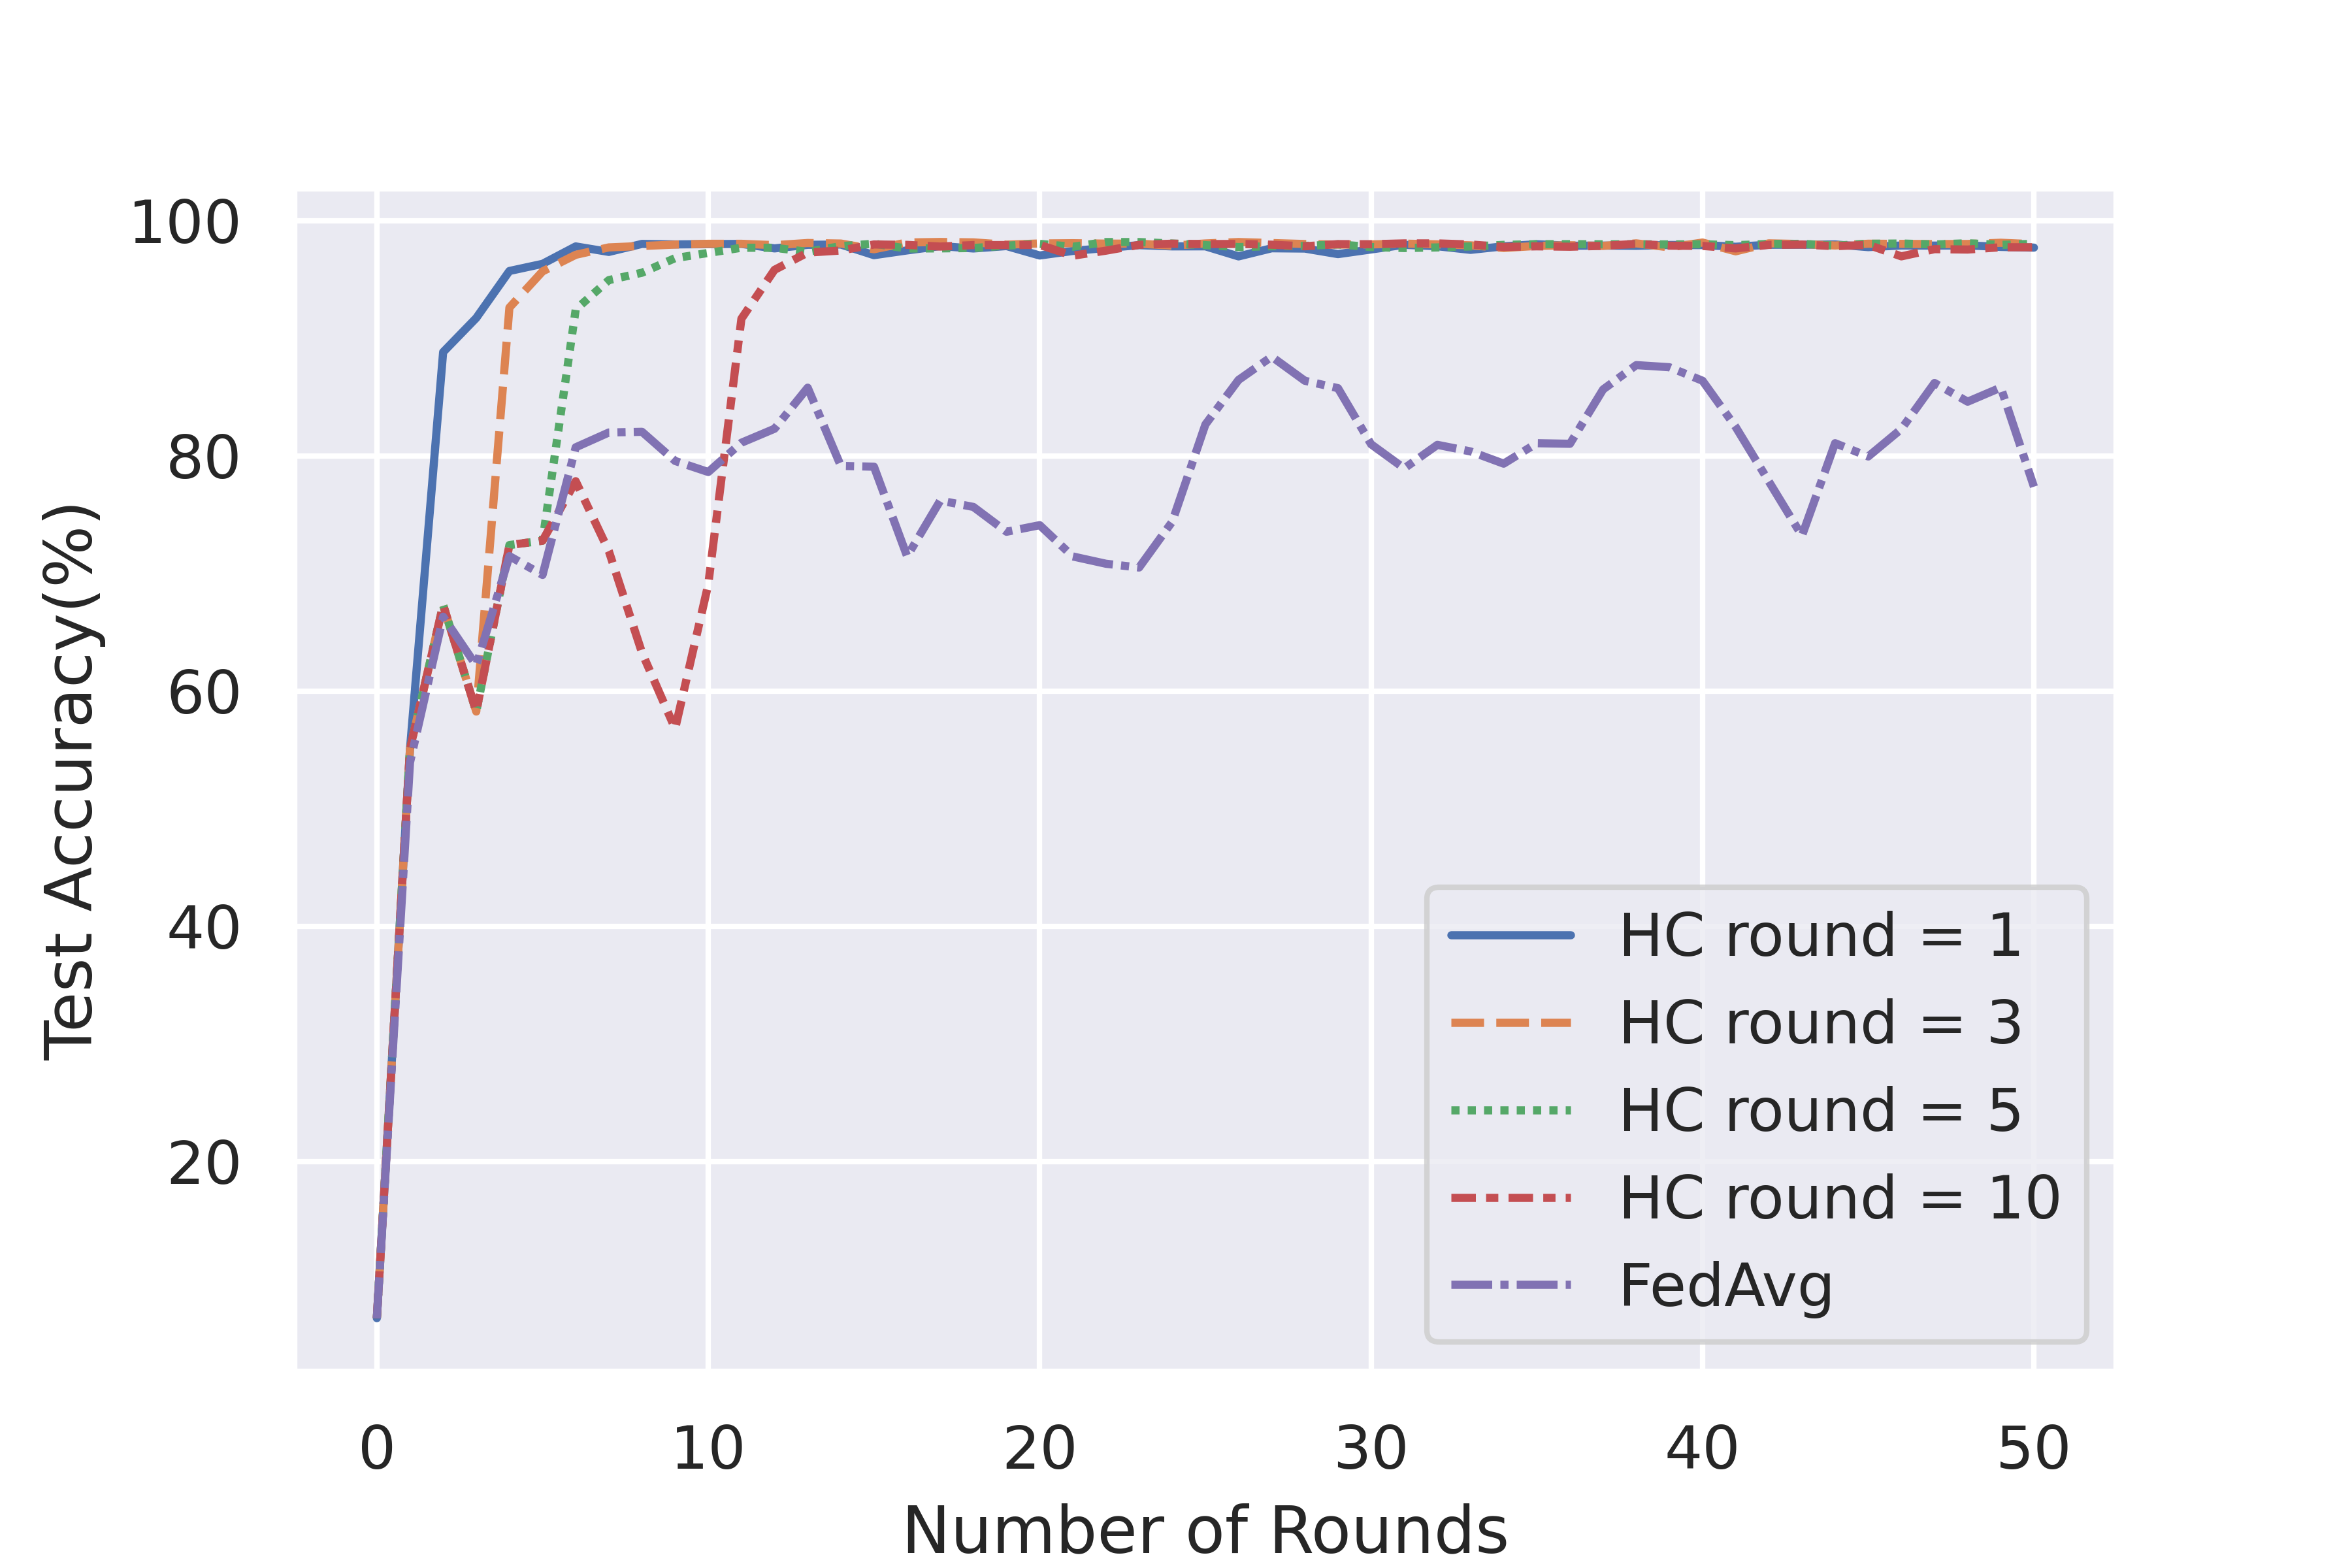
\includegraphics[scale=0.32]{figs/mnist-noniid-one-rand.png}
		\end{minipage}
	}
	\qquad
	\subfloat[MNIST数据集在标签交换的异质数据下,随训练轮次以及聚类轮次变化的的测试准确率]{
		\begin{minipage}[b]{0.27\textwidth}
			\centering
			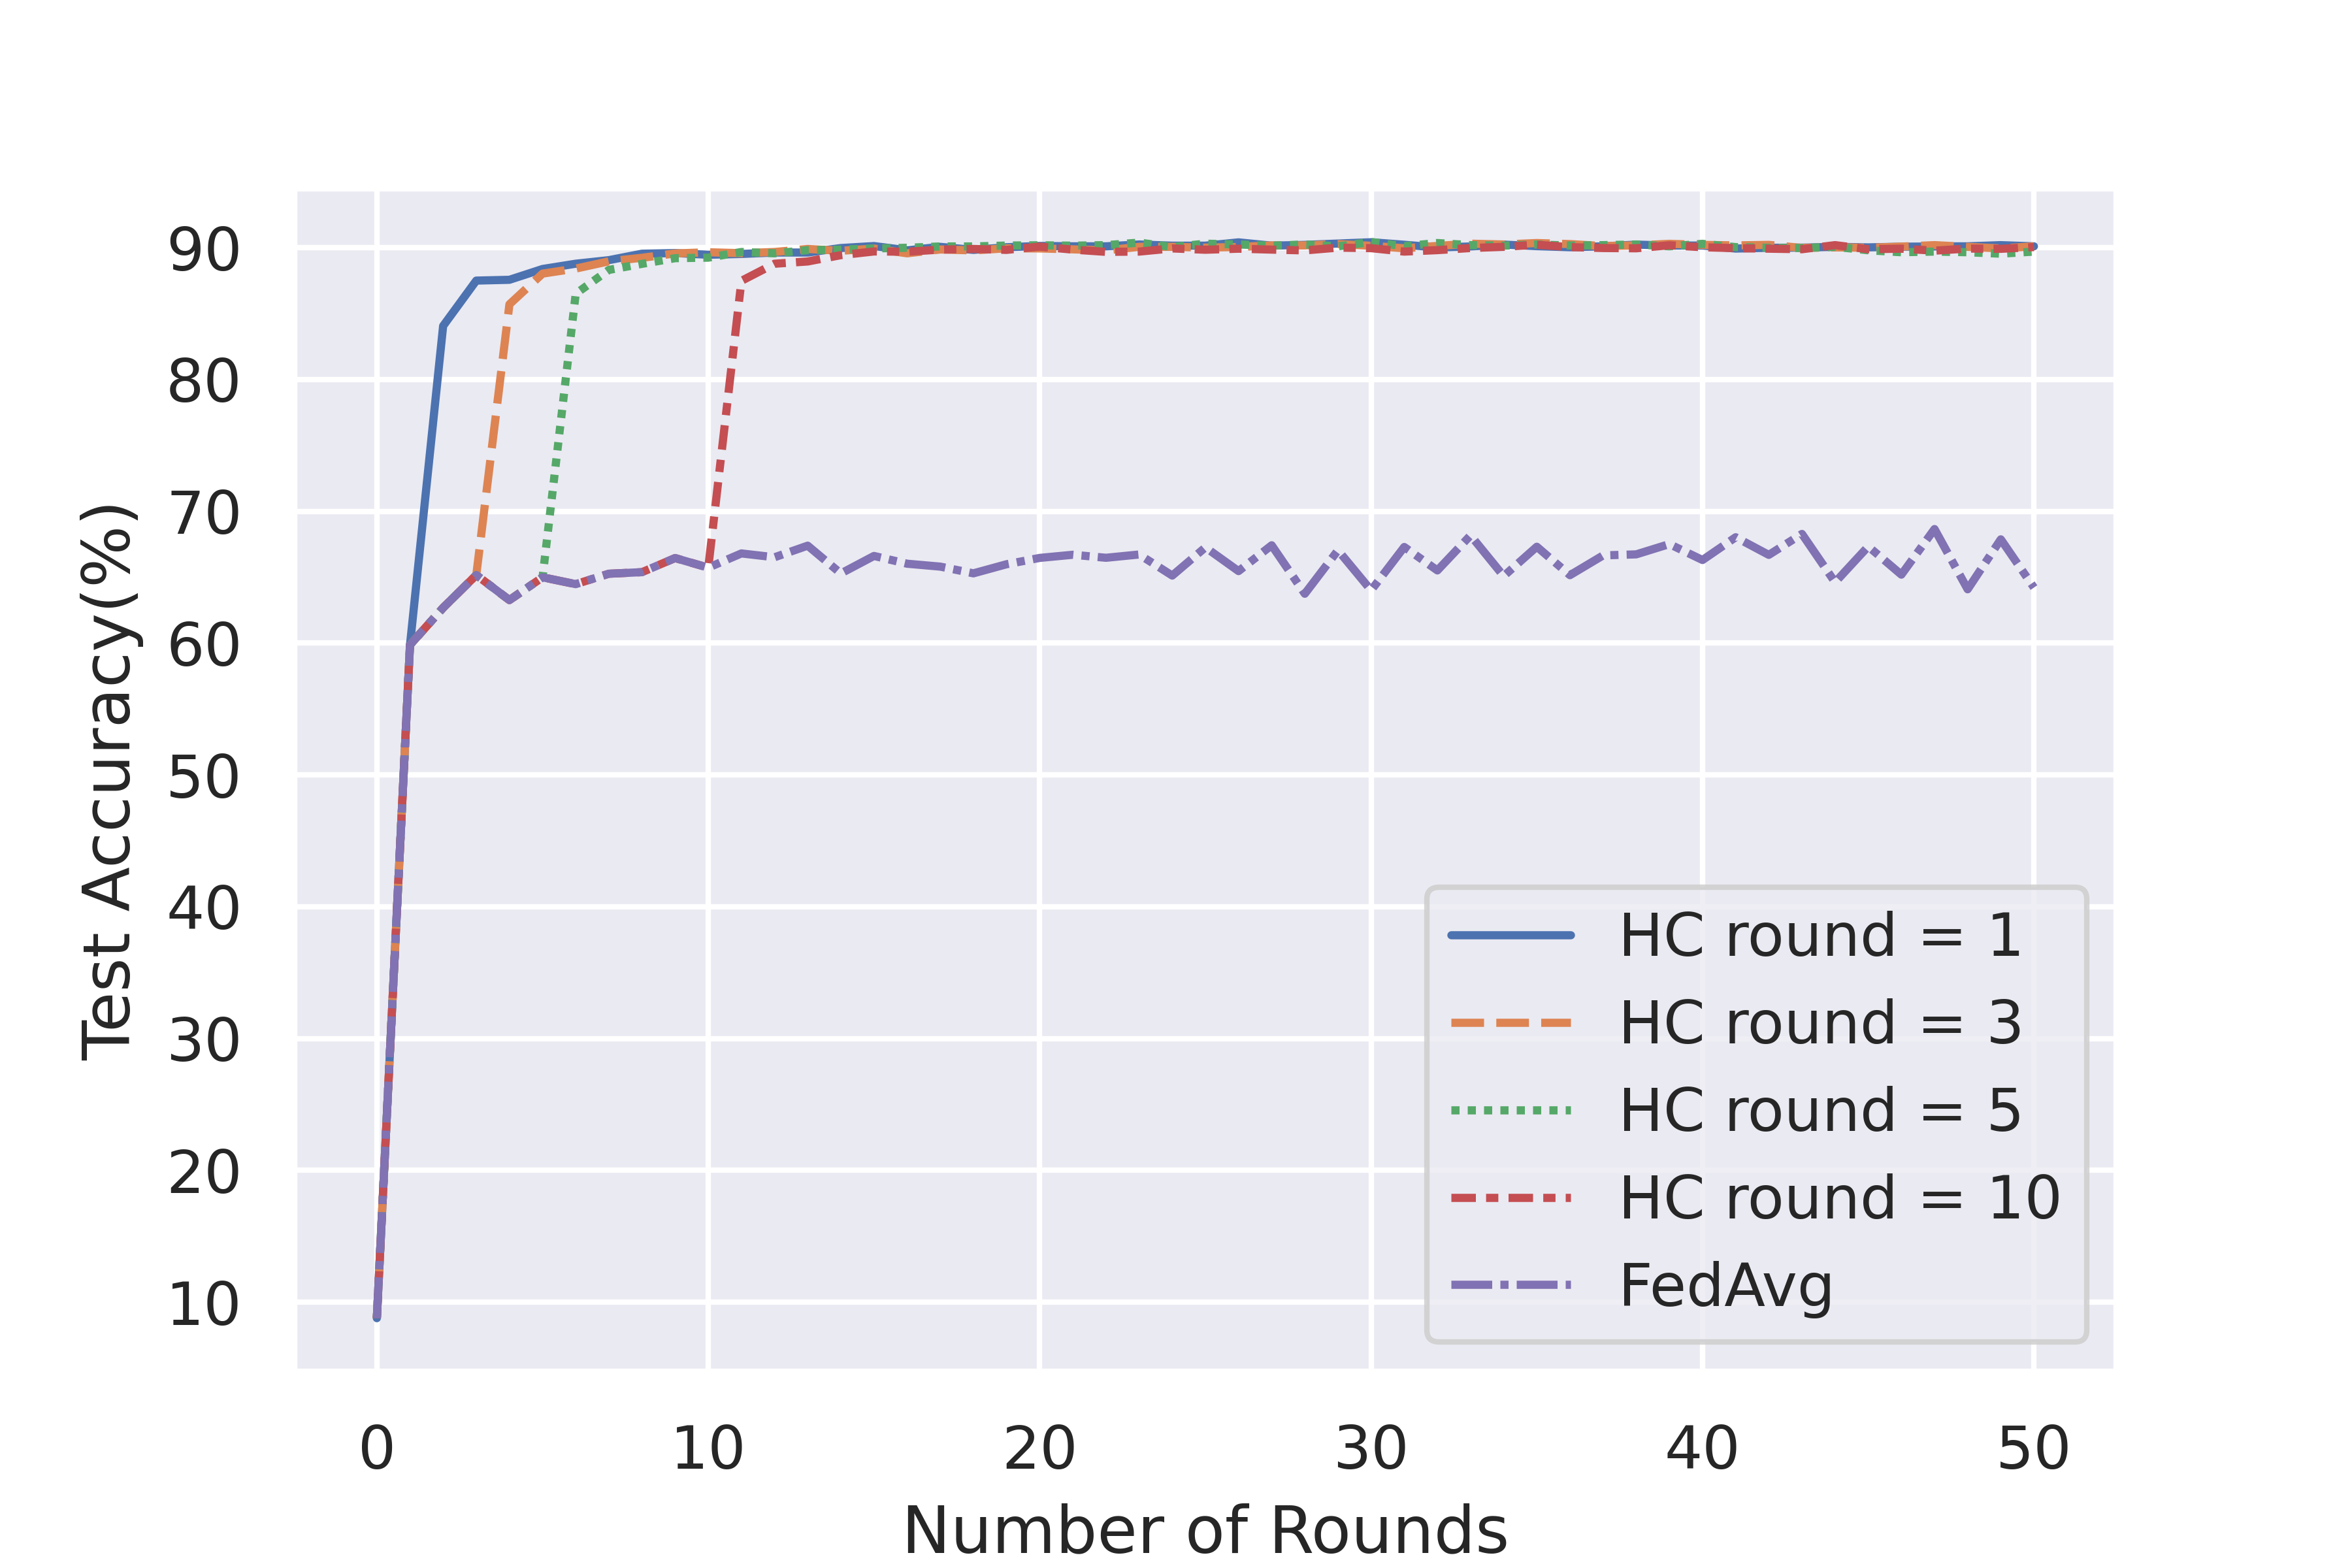
\includegraphics[scale=0.32]{figs/mnist-noniid-two.png}
		\end{minipage}
	}
	\qquad
	\subfloat[CIFAR-10数据集在分布偏差的异质数据下,随训练轮次以及聚类轮次变化的的测试准确率]{
		\begin{minipage}[b]{0.27\textwidth}
			\centering
			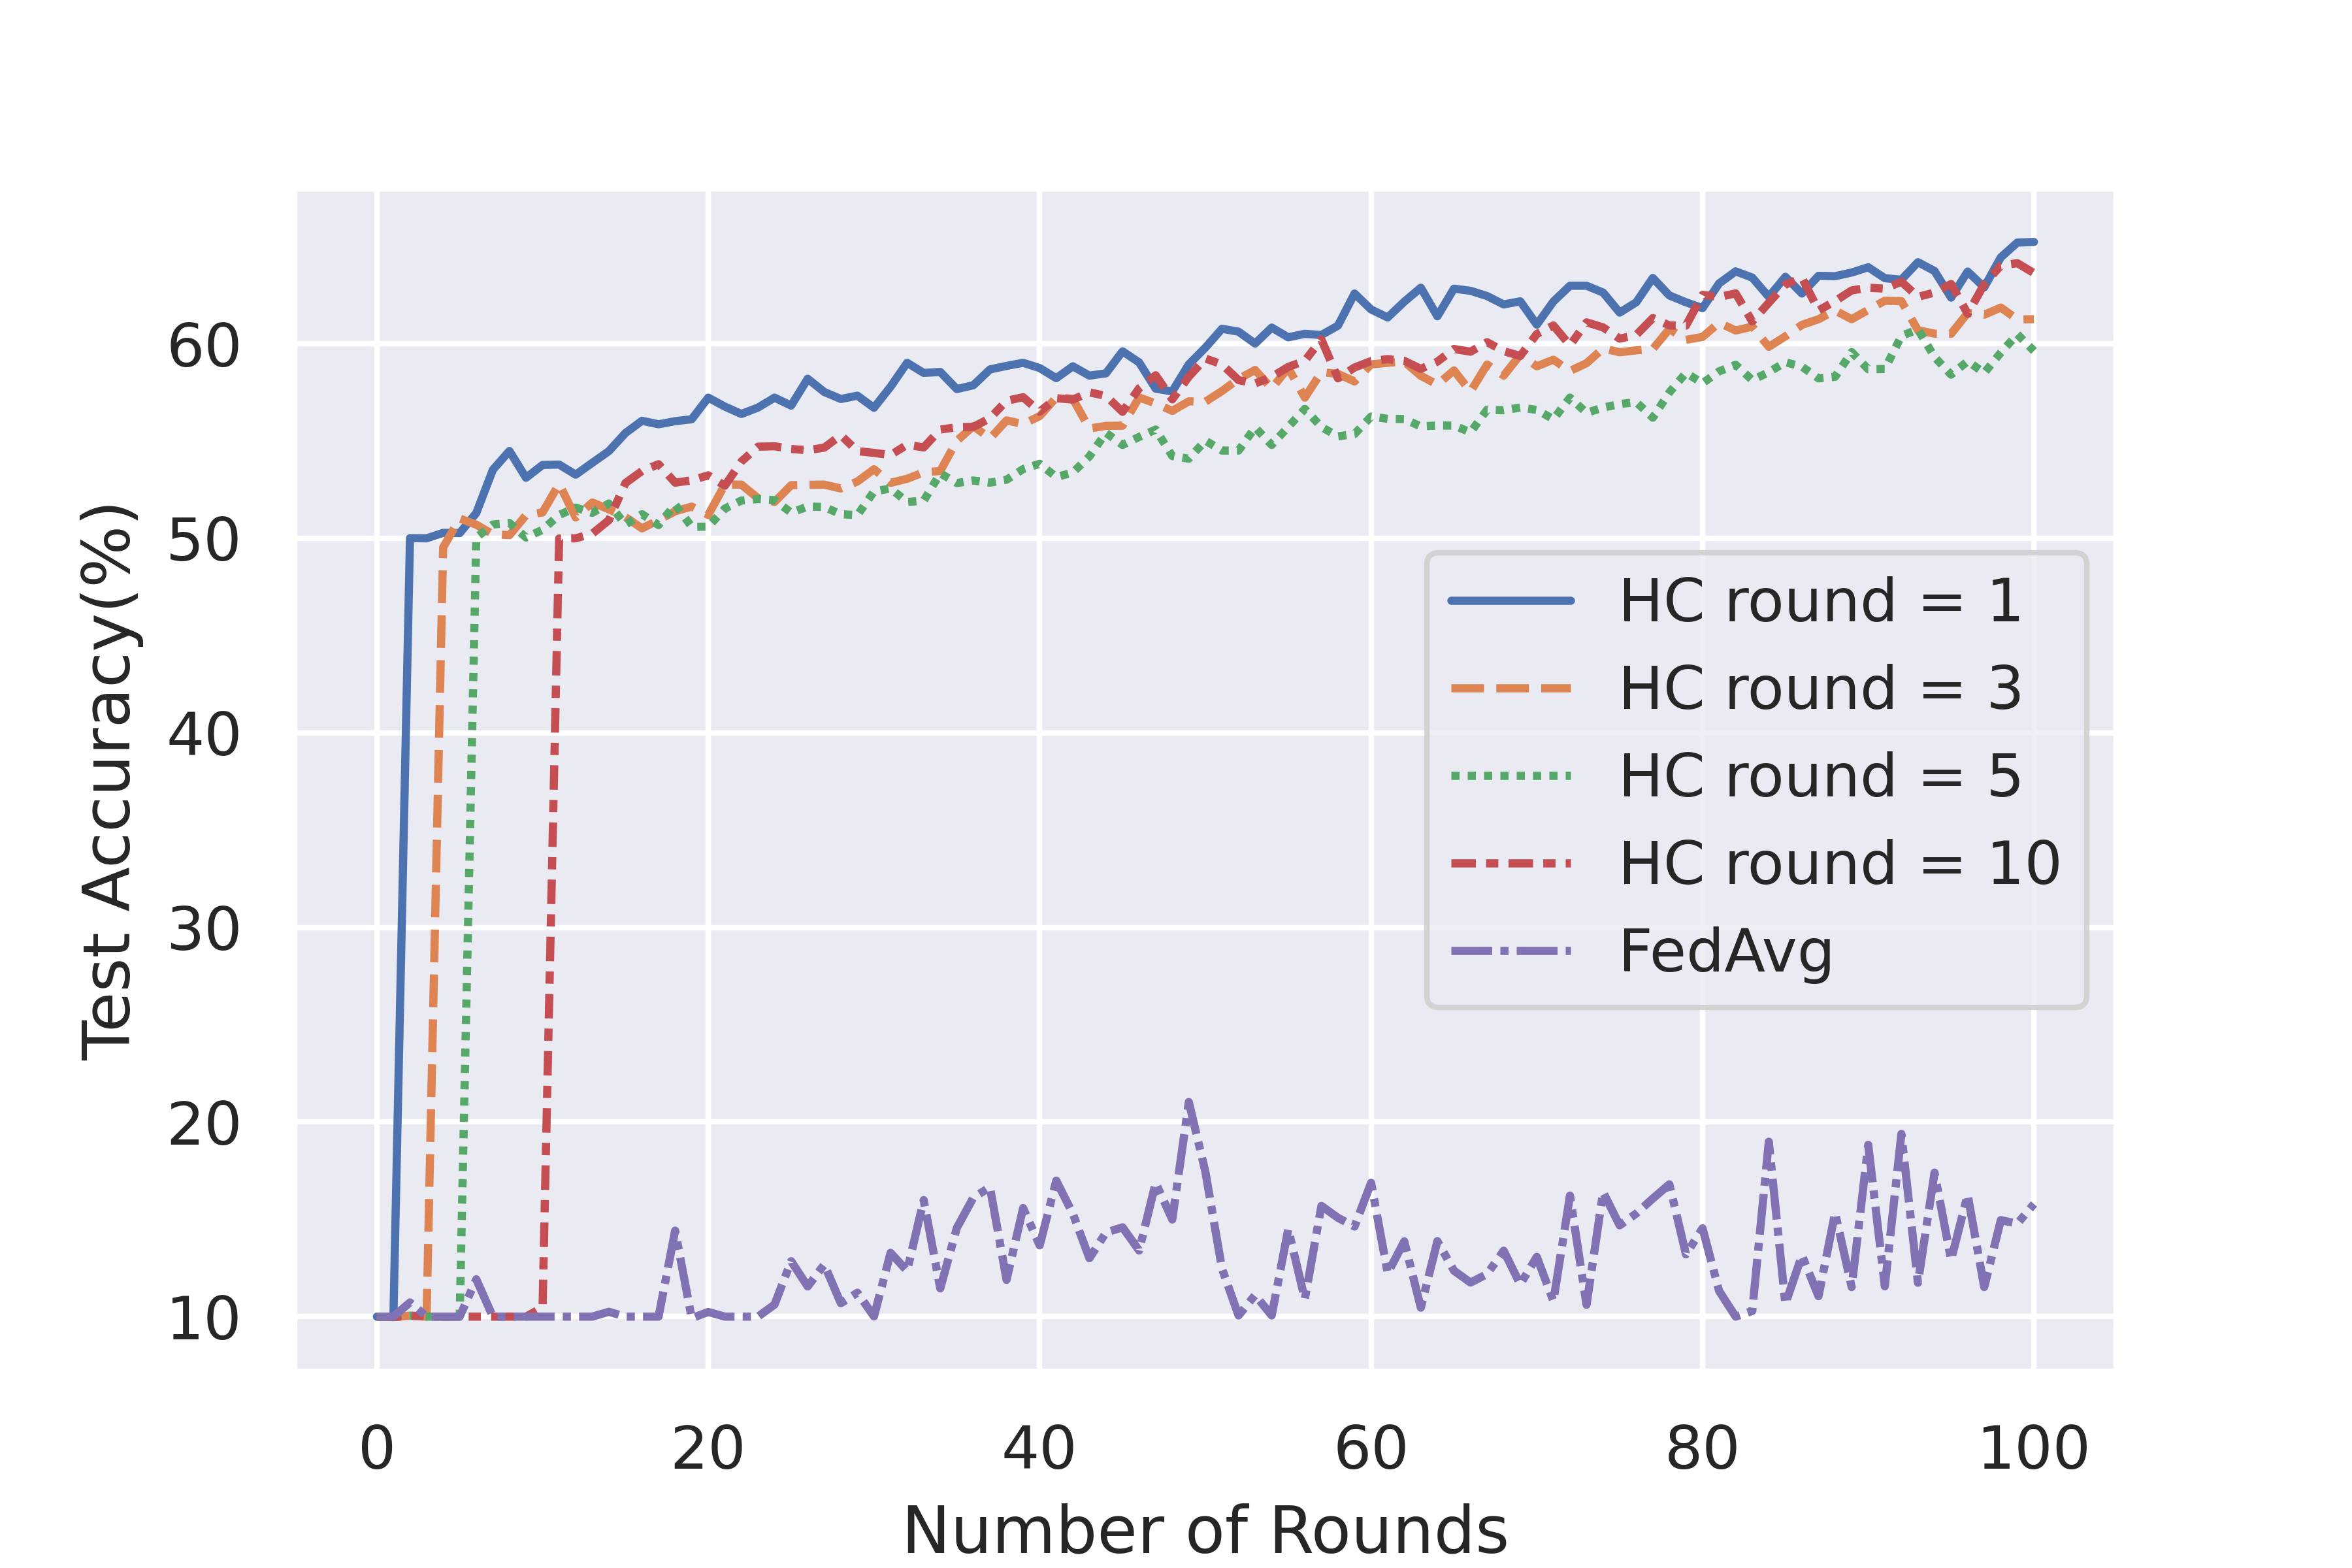
\includegraphics[scale=0.32]{figs/cifar-noniid-one-rand.png}
		\end{minipage}
	}
	\caption[方案准确率评估]{不同异质数据分布、不同训练轮次以及聚类轮次对测试准确率的影响,在(a)(b)中,使用MNIST数据集来评估. 在(c)中,使用CIFAR-10数据集来评估。}
	\label{fig-acc}
\end{figure}

% 效率测试
\begin{figure}[htb]
	\centering
	\subfloat[参与方数量变化对通信开销的影响]{
		\begin{minipage}[b]{0.45\textwidth}
			\centering
			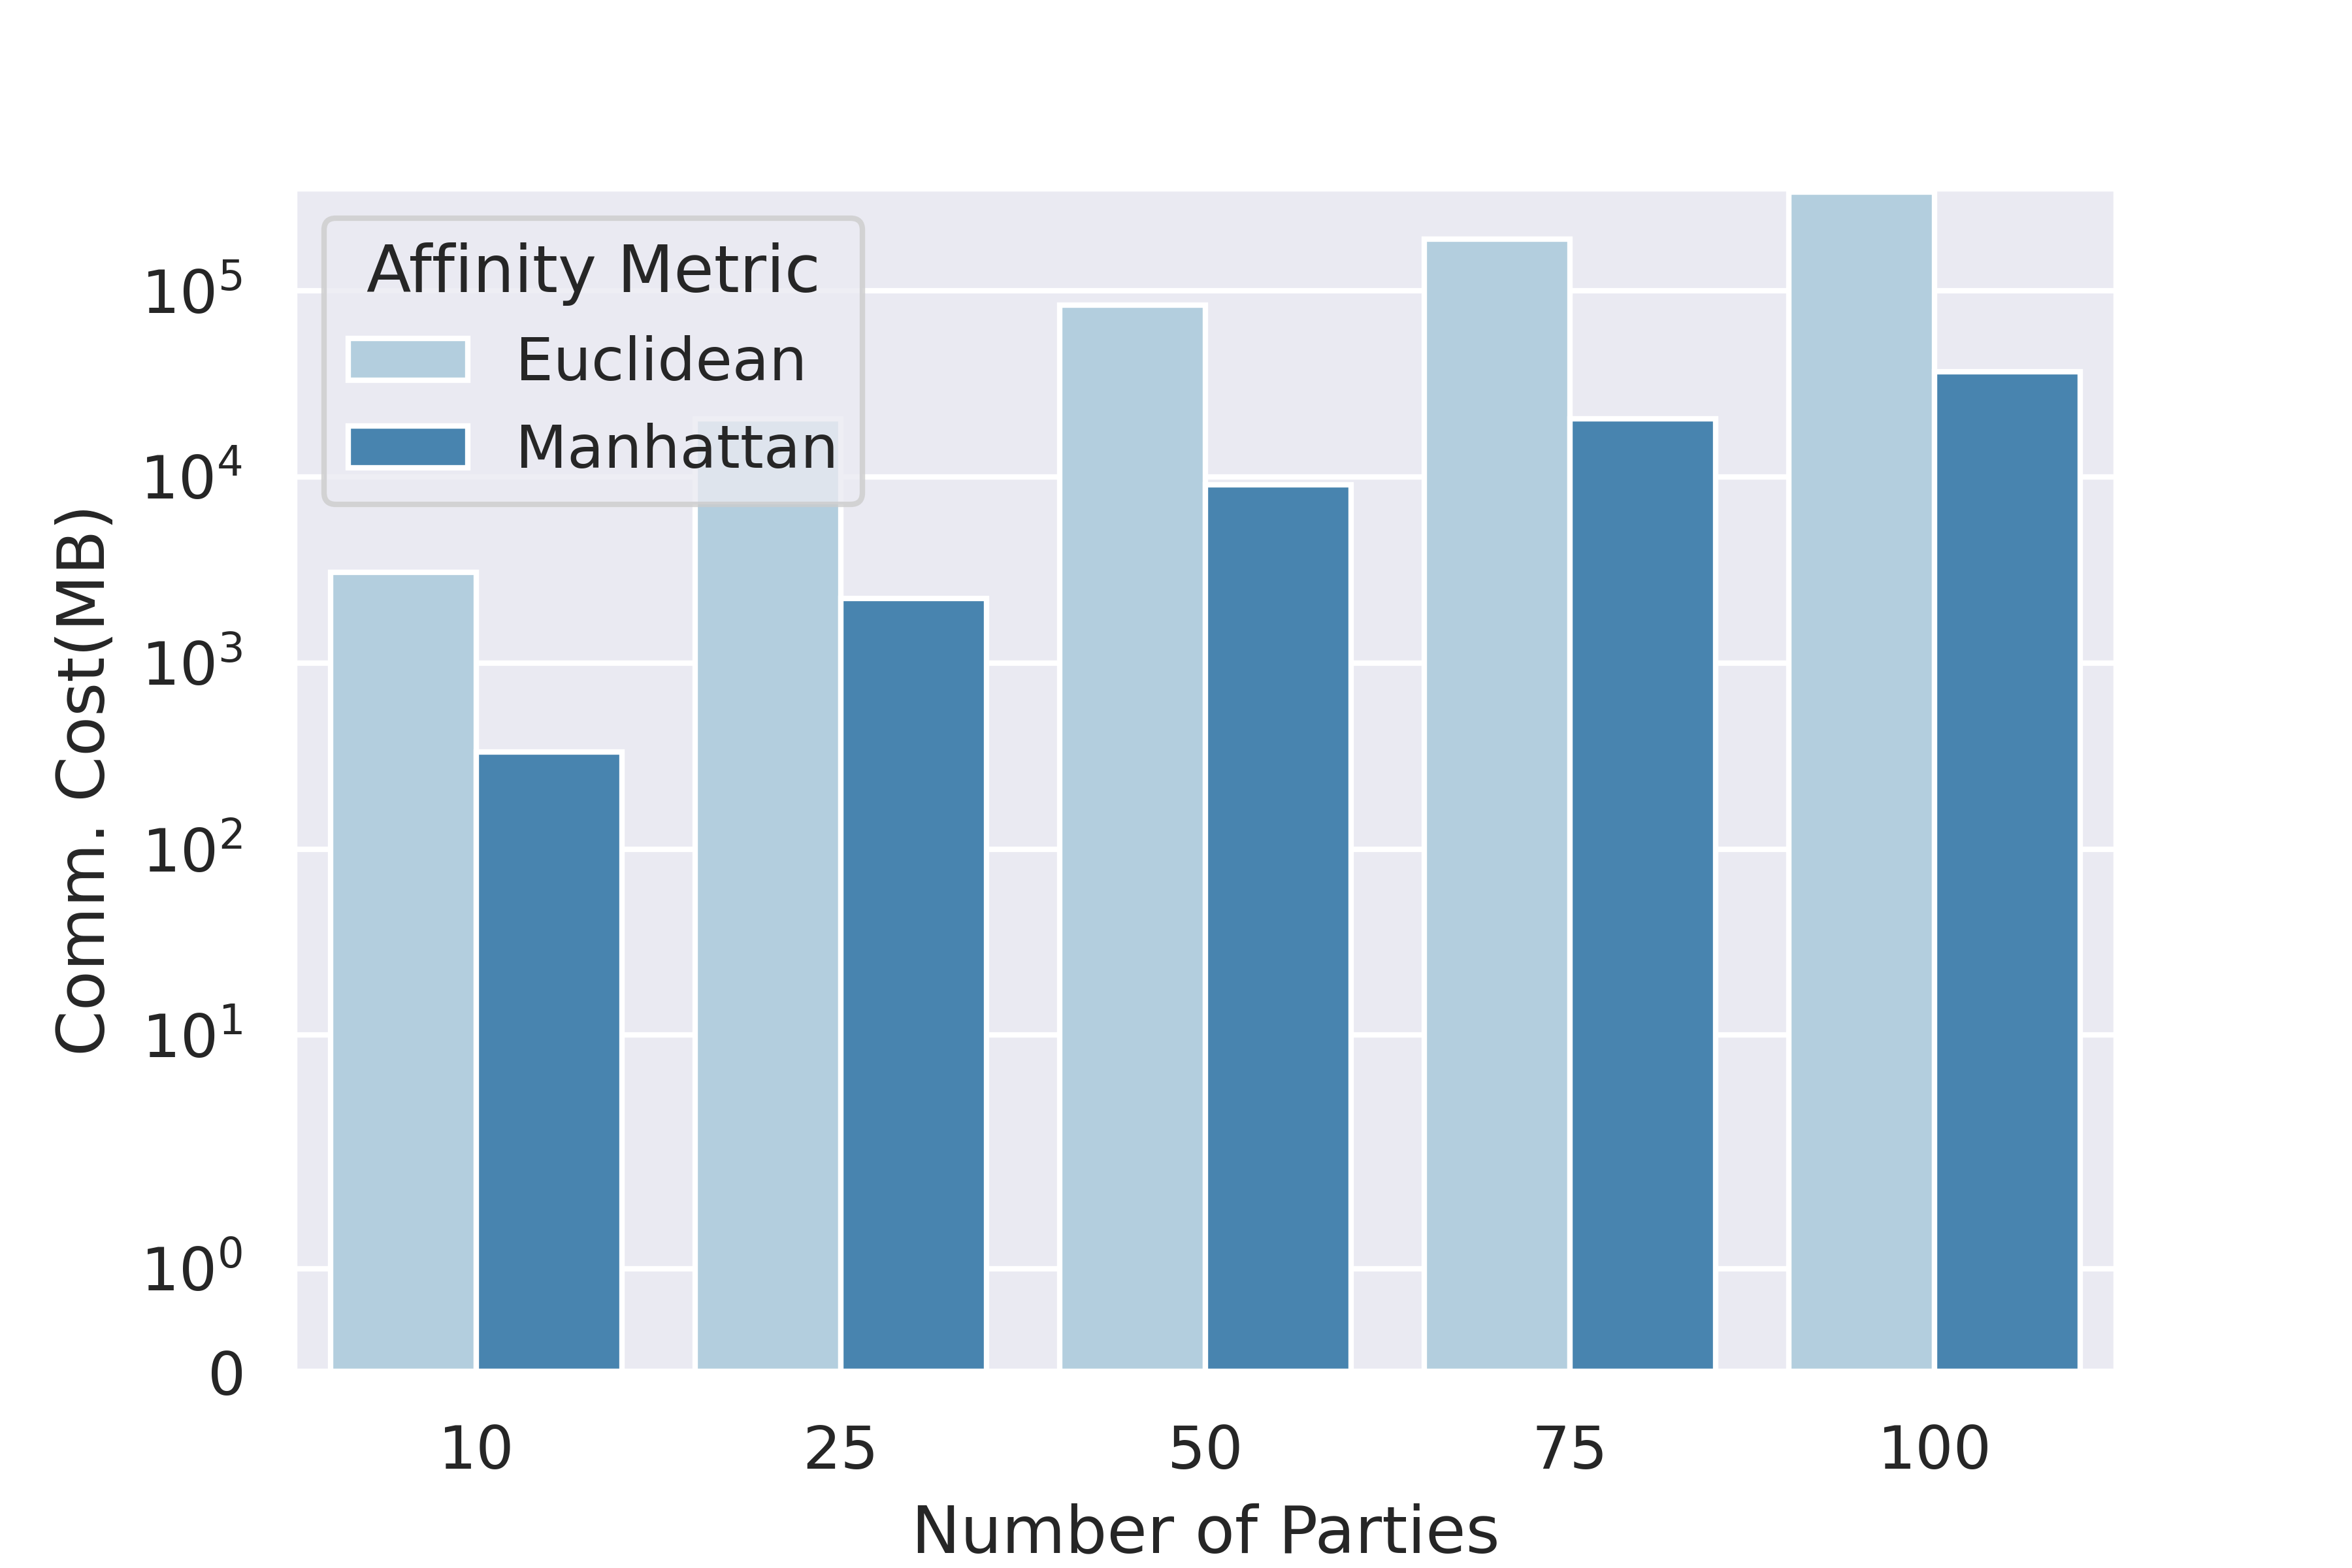
\includegraphics[scale=0.45]{figs/overheads/comm-party-79510.png}
		\end{minipage}
	}
	% \hspace{-1.0in}
	\qquad
	\subfloat[参与方数量变化对执行时间的影响]{
		\begin{minipage}[b]{0.45\textwidth}
			\centering
			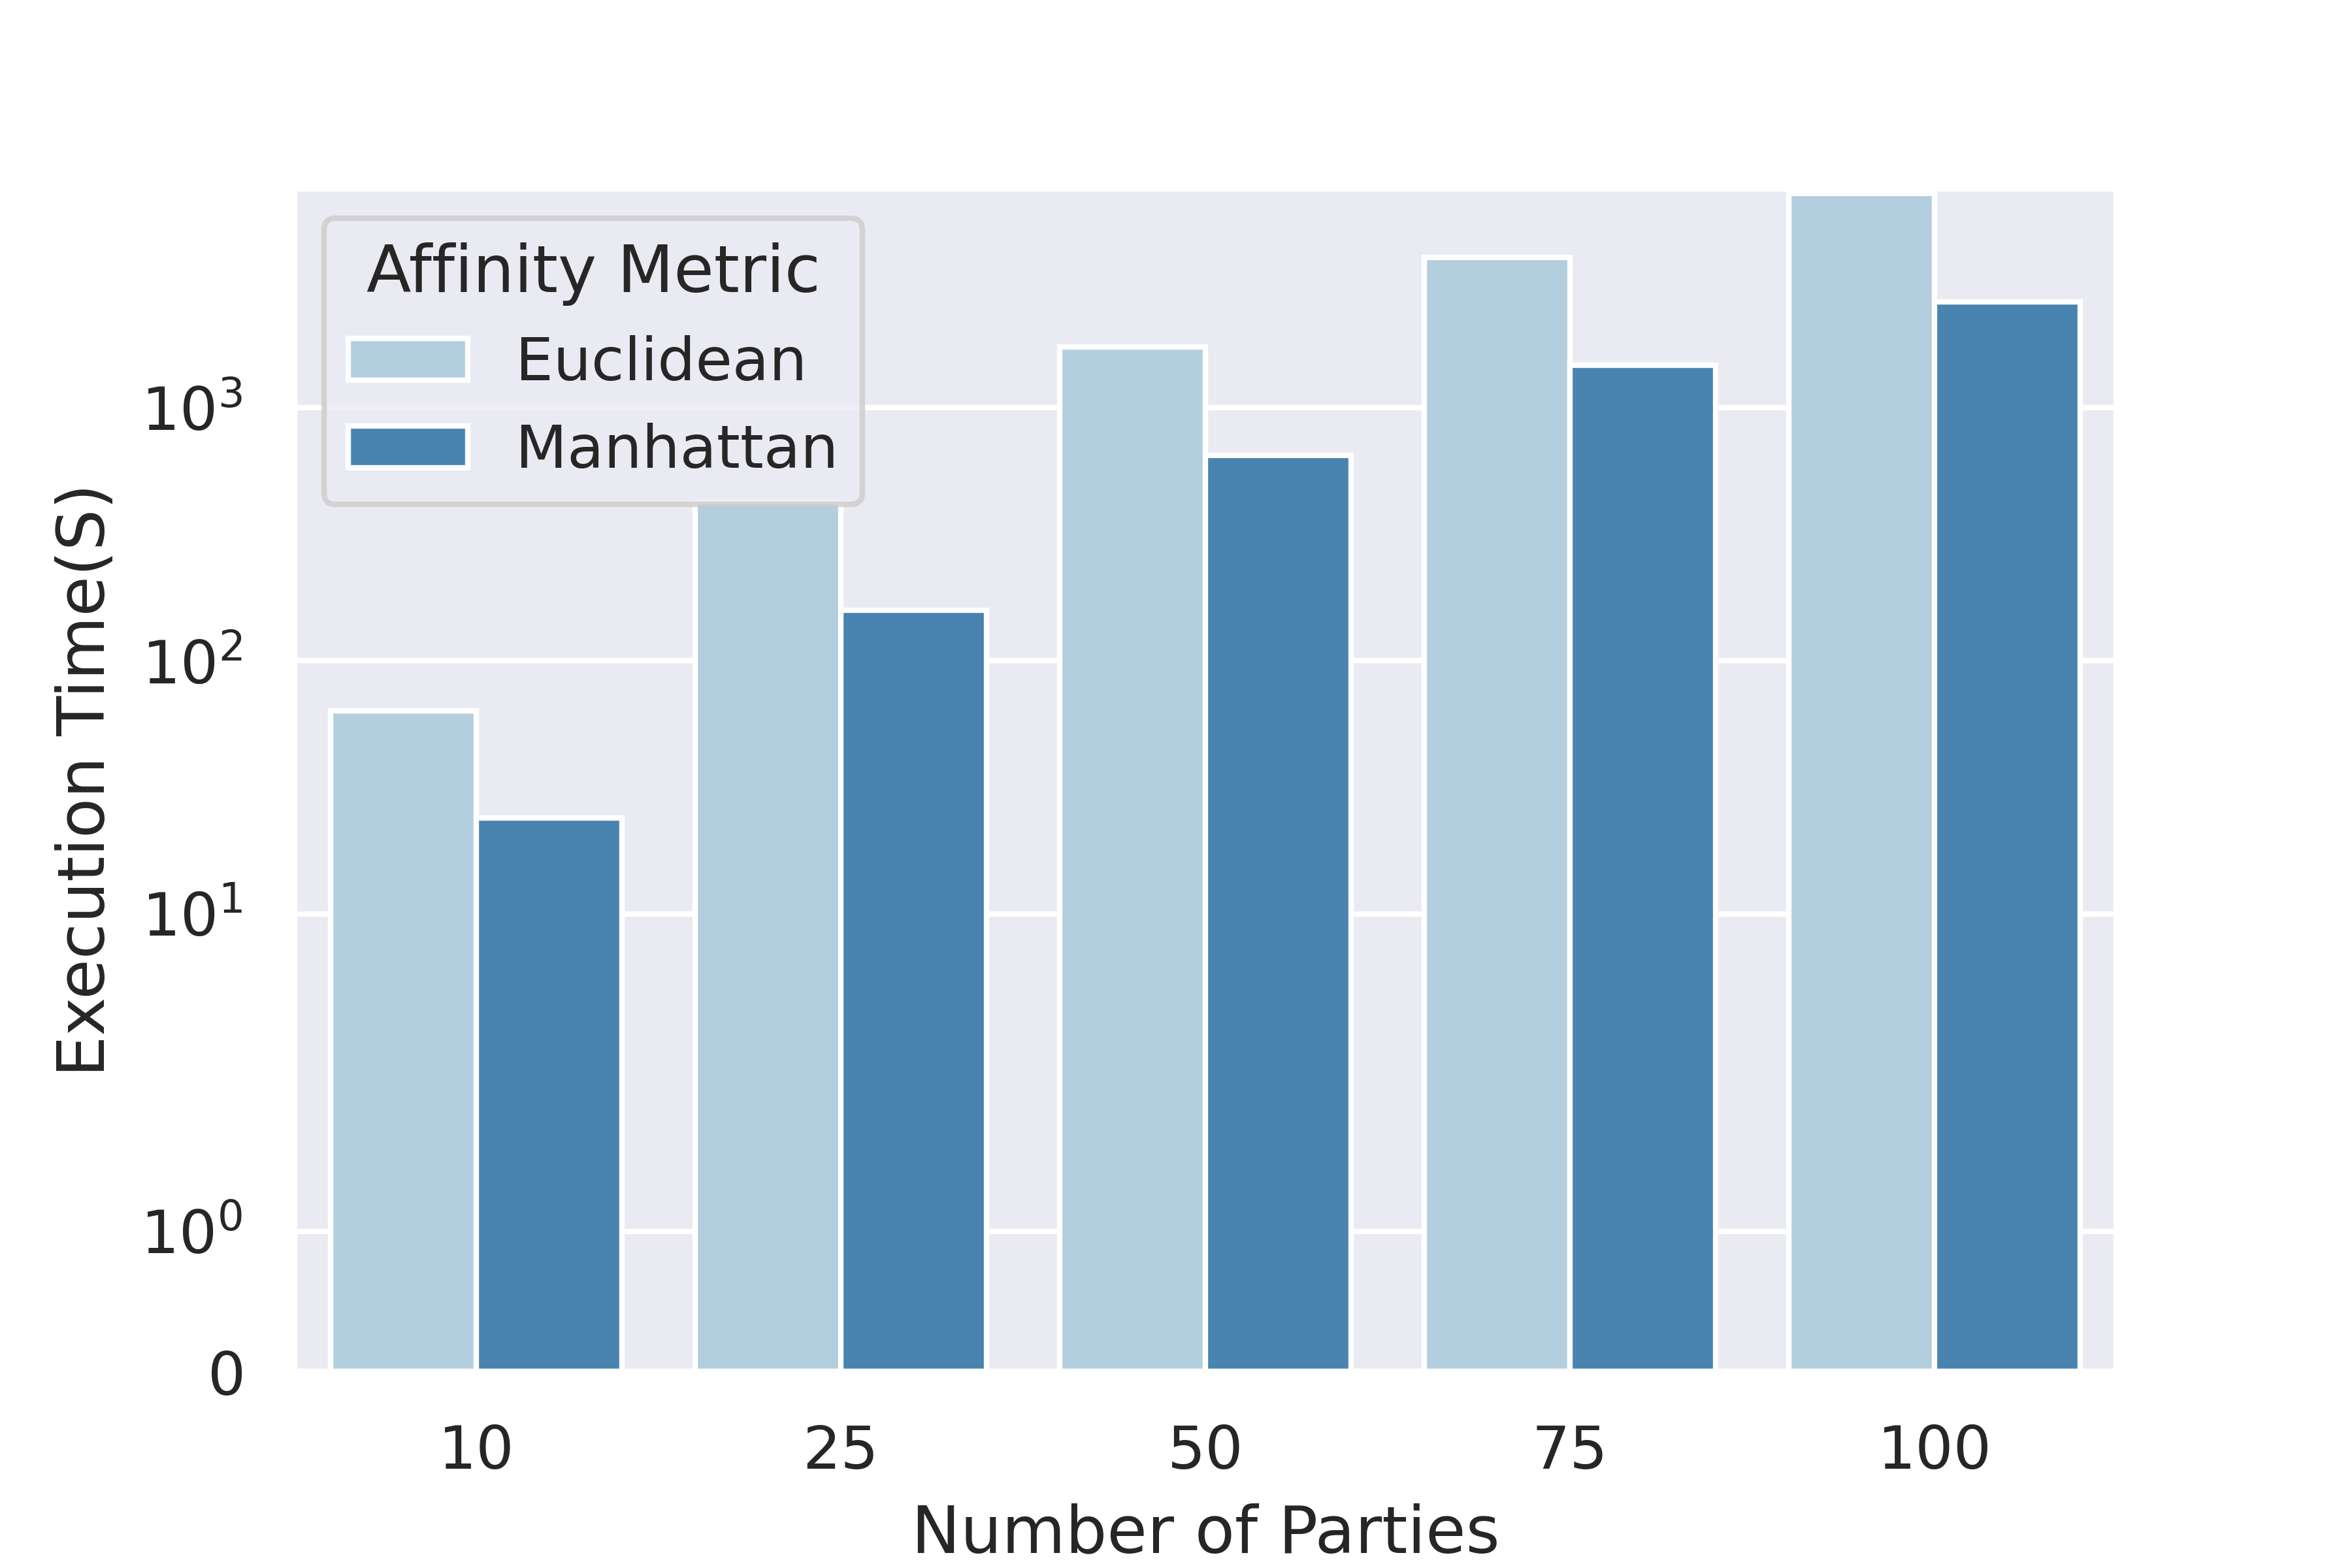
\includegraphics[scale=0.45]{figs/overheads/time-party-79510.png}
		\end{minipage}
	}
	\qquad
	\subfloat[不同输入维度对通信开销的影响]{
		\begin{minipage}[b]{0.45\textwidth}
			\centering
			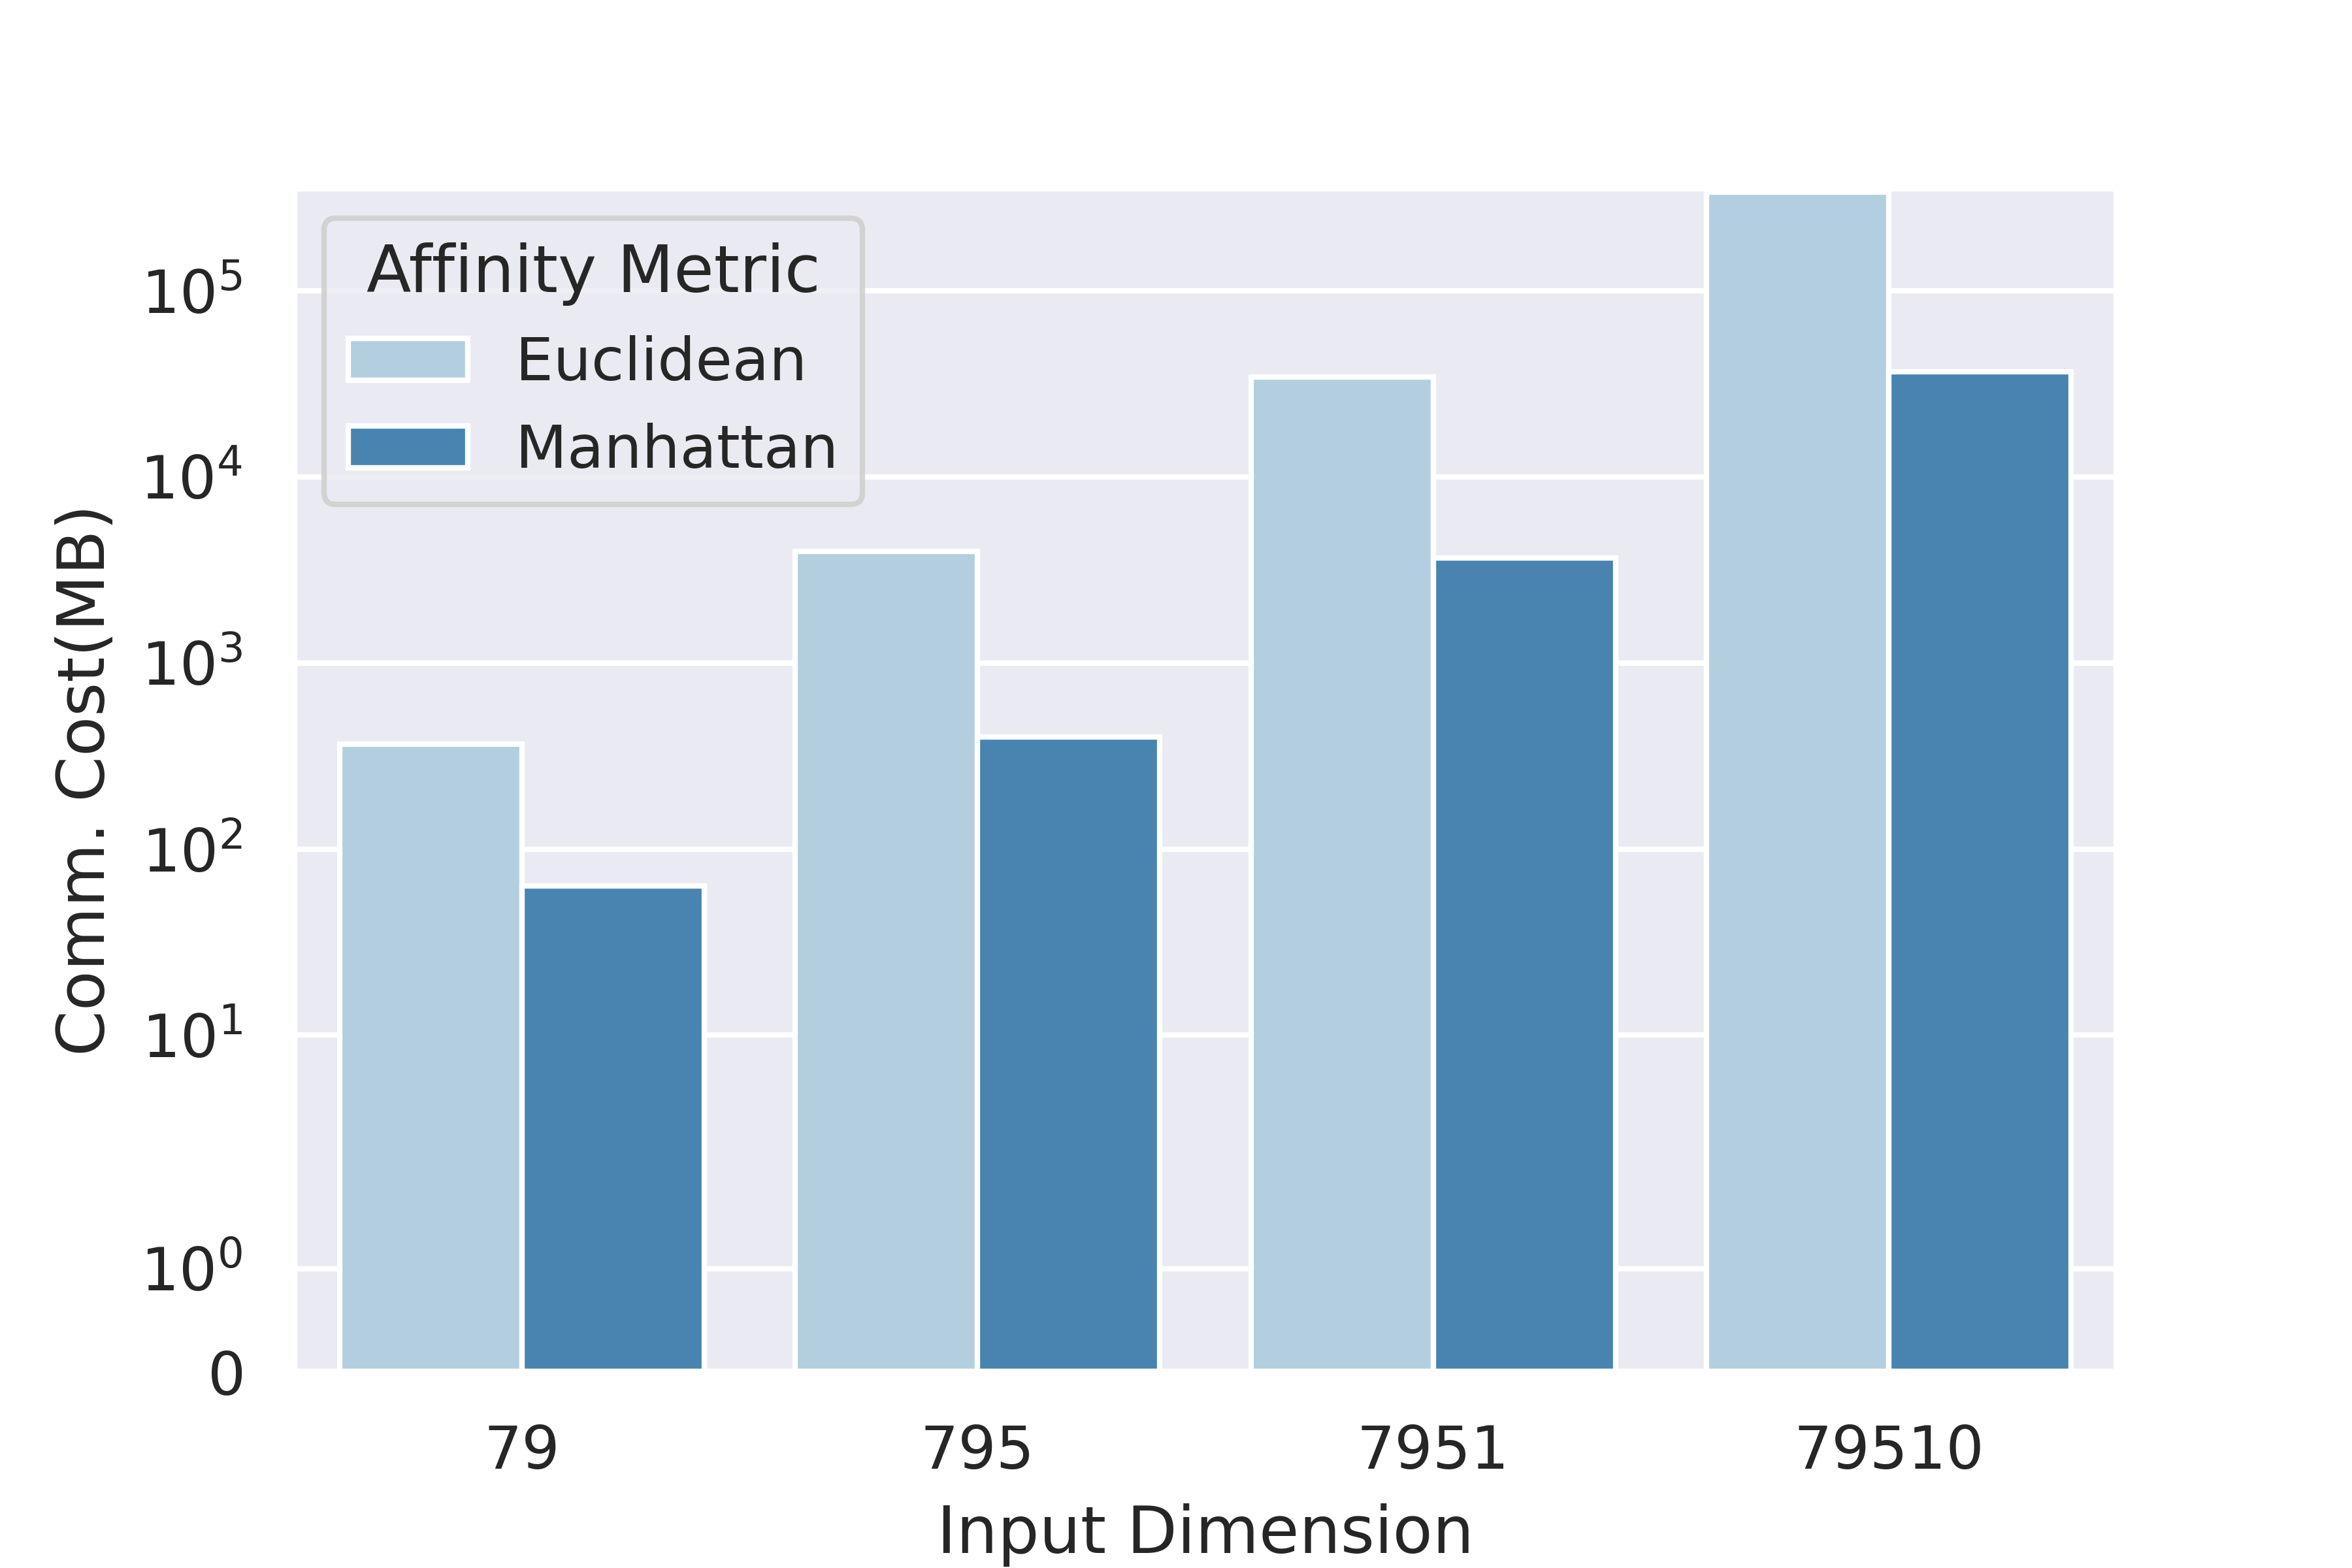
\includegraphics[scale=0.45]{figs/overheads/comm-dimension-100.png}
		\end{minipage}
	}
	\qquad
	\subfloat[不同输入维度对执行时间的影响]{
		\begin{minipage}[b]{0.45\textwidth}
			\centering
			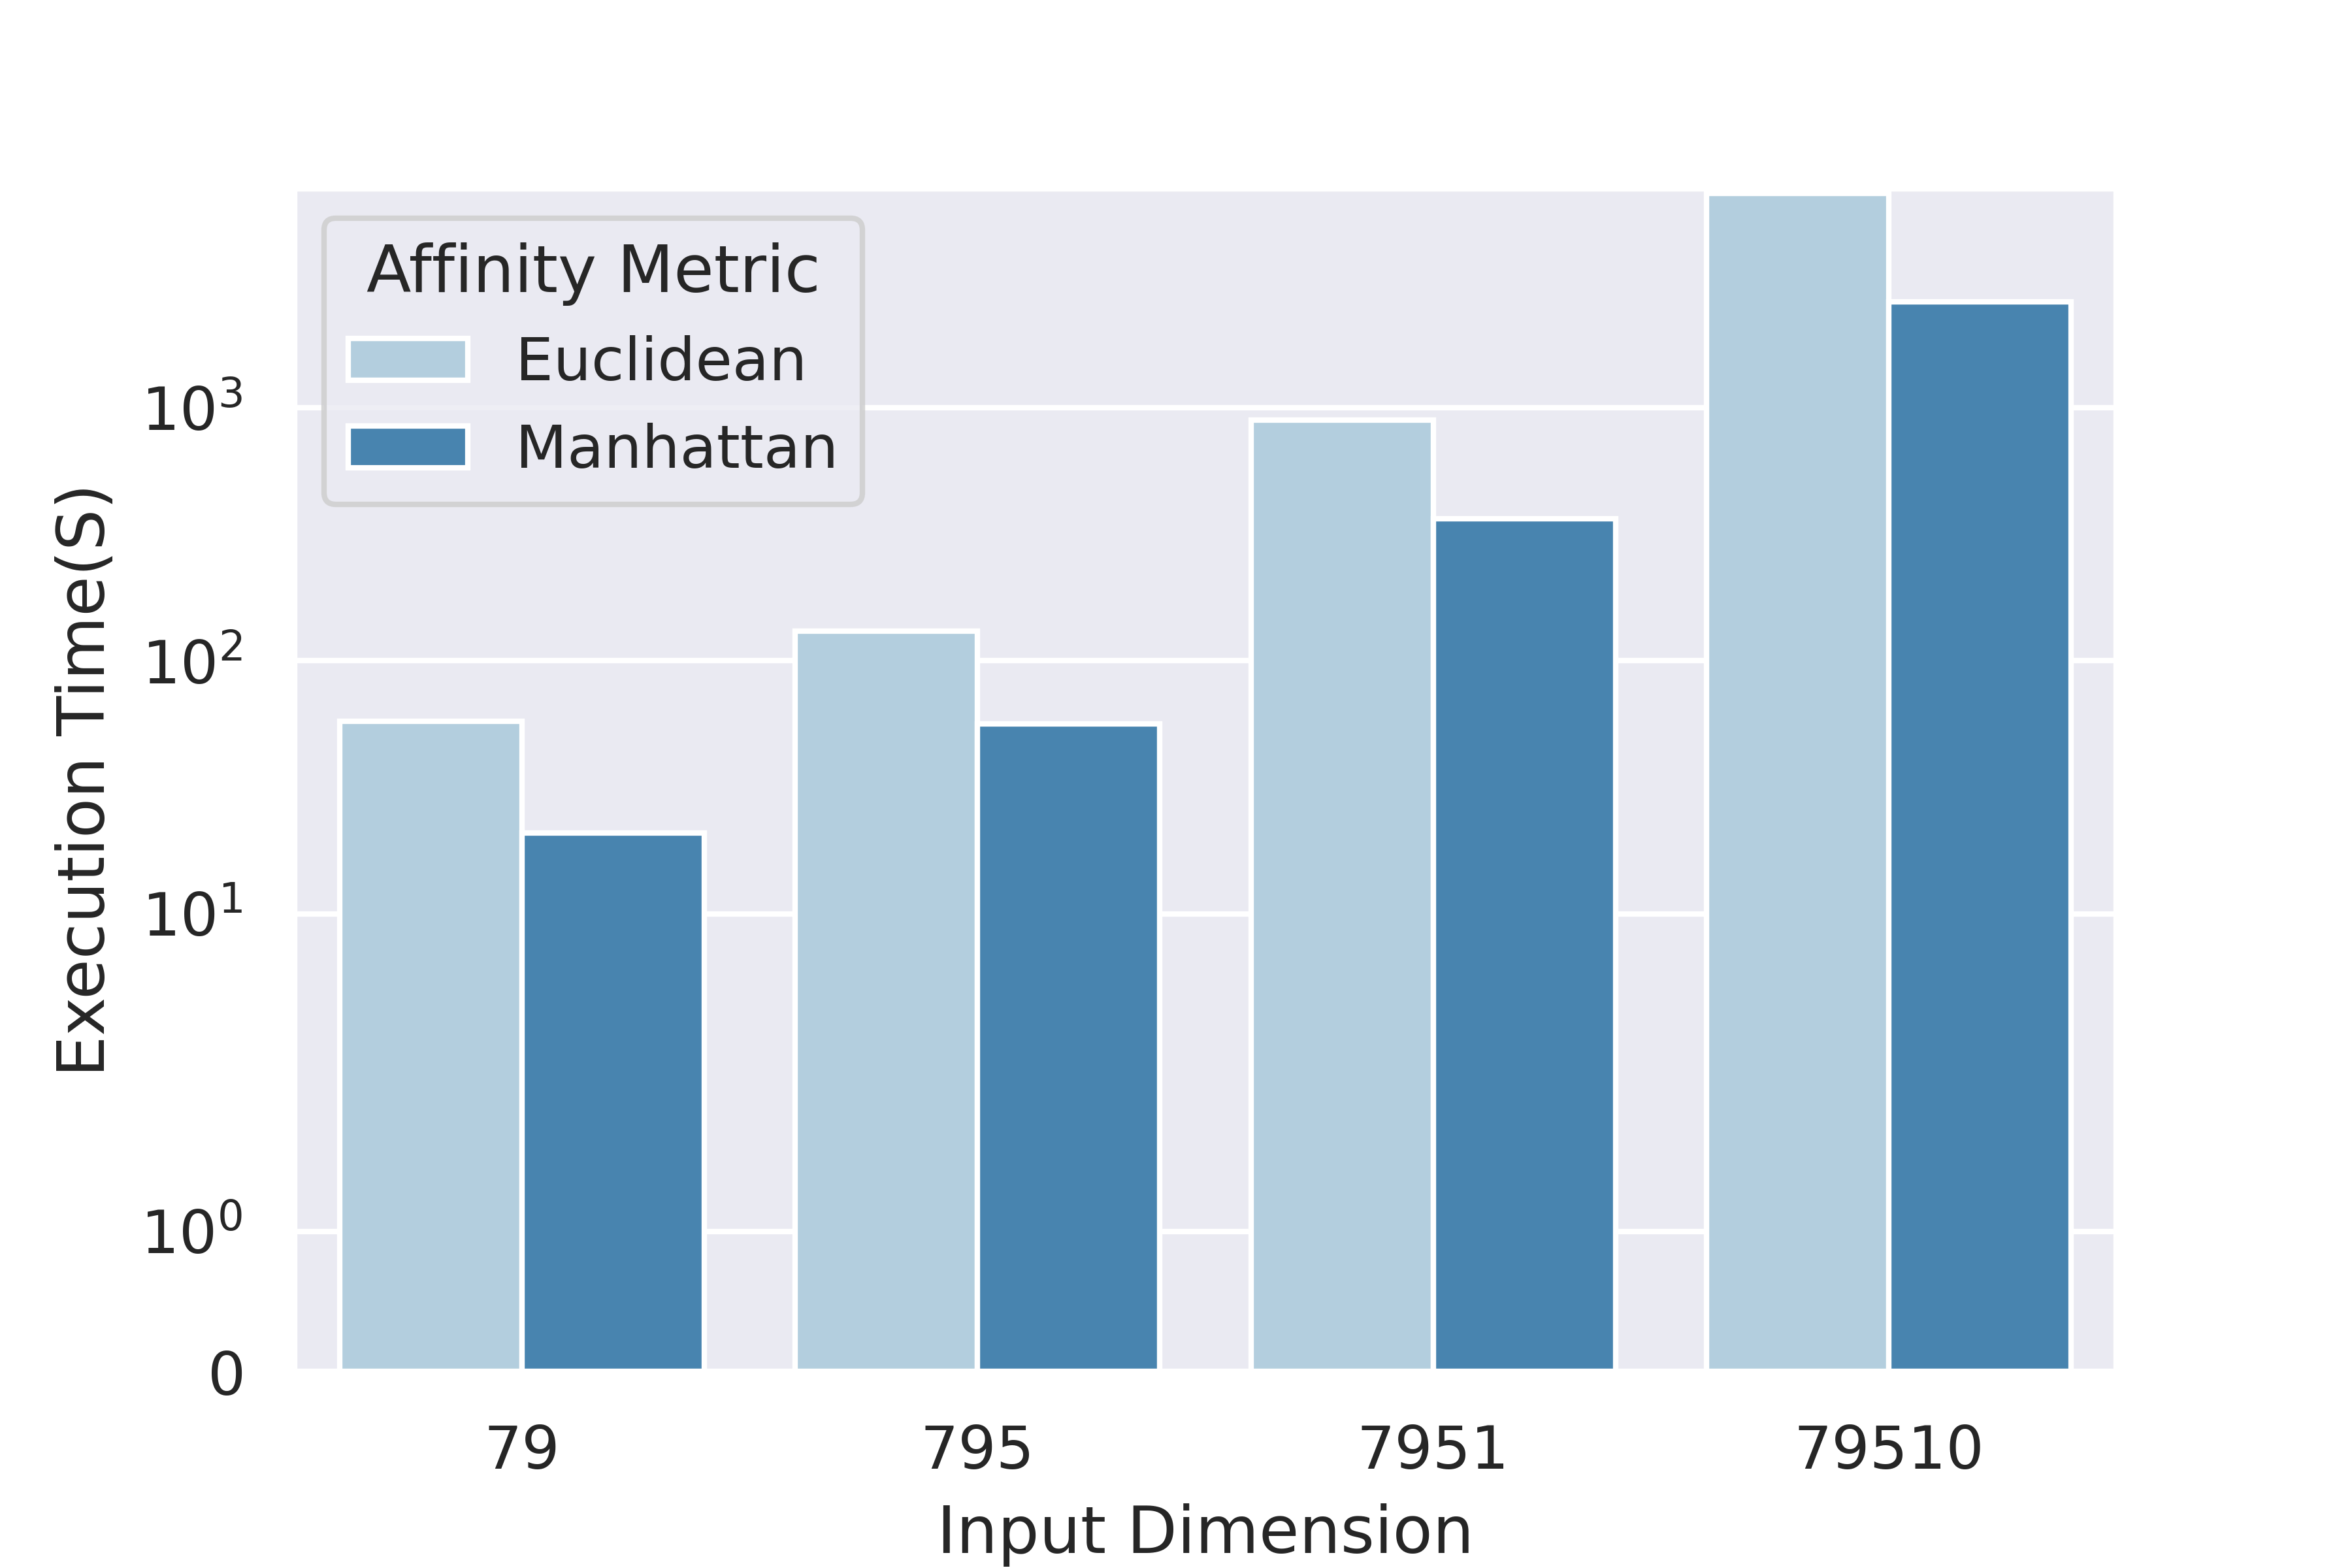
\includegraphics[scale=0.45]{figs/overheads/time-dimension-100.png}
		\end{minipage}
	}
	\caption[方案效率评估]{不同的安全距离度量方式、不同参与方以及不同输入维度对本方案通信开销以及执行时间的影响,在(a)(b)中,梯度维度固定为79510,在(c)(d)中,参与方的数量被固定为100。}
	\label{fig-cost}
\end{figure}

\subsubsection{准确率测试}

许多因素会影响全局模型的准确率,其中包括神经网络模型的容量,参与方数据的数量和质量以及训练的轮次等等,而我们关注的是本方案在数据分布为异质的情况下,对比经典FedAvg算法联合训练准确率的提升。
因此我们变化聚合轮次,探究聚类操作的时机对全局模型准确率的影响。
注意因为我们对CIFAR-10分类任务使用的网络结构相对简单,所以整体上准确率偏低,这是因为我们的重点在于对比FedAvg性能的提升。

\textbf{不同异质数据类型的影响:}图片\ref{fig-acc} 展示了不同数据集(MNIST和CIFAR-10)在不同异质数据场景下,不同的聚类轮次对于联合训练准确率的影响。
我们观察到所有数据集在所有的异质数据分布场景,在聚类轮次之后,都有较大的训练准确率的上升(1.13-5.0 $\times$ FedAvg)。其中CIFAR-10数据集在分布偏差的异质数据中准确率增长最明显(5.0 $\times$ FedAvg),同时所有的情况下的在收敛后都能得到很好的测试准确率。
这表明我们的安全层次聚类算法(SHC),可以很好的将拥有相似的梯度的参与方分为一个簇,在同一个簇内联合生成全局模型,很好的避免了目标不一致梯度的影响,因此提高了整体全局模型的性能。

\subsubsection{效率测试}
本方案性能瓶颈在于层次聚类过程中需要计算一次的梯度之间的相互距离,对于$n$个参与方,每个参与方梯度维度为$d$,其计算复杂度是 $O(n^2)\times d$。
于是我们单独对距离矩阵的计算做了效率评估,包括对通信开销的评估和执行时间的评估。

\textbf{参与方数量的影响:}在图片\ref{fig-cost}(a)和 图片\ref{fig-cost}(b)中,我们把梯度的维度固定为 $79510$(MNIST网络模型参数的维度),然后观察不同参与方数量对通信开销和执行时间的影响,我们发现随着参与方数量的增加,通信开销和执行时间都有比较大的增加。其中对比不同的距离度量方式(欧式距离或者曼哈顿距离),我们观察到使用曼哈顿距离比使用欧式距离,在通信开销上有 $8.23 \times$ 的提升,在执行时间上有 $1.67 \times$ 的提升。这是因为我们设计的SMD算法\ref{alg2}不涉及到开销更大的安全乘,更加轻量。

\textbf{不同梯度维度的影响:}为了减少安全距离矩阵计算的通信开销和执行时间开销,同时保证高的聚类精度,我们将将梯度按照百分比在聚类前进行随机的降维操作。在图片\ref{fig-cost}(c)和图片\ref{fig-cost}(d)中,我们逐步减少梯度的维度,同时比较聚类结果,发现当梯度的维度降低到100这个数量级时(MNIST梯度维度为79),保证了聚类精度的同时,最大限度的减小了计算和通信开销。这是因为梯度的维度较高,裁减了维度之后还能保持较好的特征,所有还是可以被层次聚类很好的分类。对比距离度量方式,我们观察到曼哈顿距离作为度量方式对比欧式距离,在通信开销上有 $4-78-8.93 \times$ 的提升,在执行时间上有 $1.56 \times$ 的提升。


\section{本章小结}\label{4-conclusion}
本章提出了一个新颖的联邦学习框架,在保证参与方本地数据隐私和全局梯度隐私的前提下,实现了较高的异质数据联合训练准确率。本方案提出了高效的基于秘密共享的安全计算模块,其中包括SED、SMD、SHC和SGB。除此之外,我们在真实数据集上对两种极致的异质数据分布进行了实验,证明了本方案在保证隐私的同时提升了异质数据联合训练的准确率。

本方案改造自FL+HC\cite{briggs2020federated},实现了对梯度的完全隐私保护,但是本方案也继承了FL+HC的缺点,即层次聚类的结果对全局模型的影响较大。还有一个限制是我们的框架需要两个不共谋的服务器,要实现单服务器的安全层次聚类更加有挑战性的安全计算协议设计,同时也会遇到更多的性能瓶颈,我们将这些问题的解决作为未来的工作方向。